\documentclass[conference,a4paper]{IEEEtran}
\usepackage{cite}
\usepackage{amsmath,amssymb,amsfonts}
\usepackage{graphicx}
\usepackage{booktabs}
\usepackage{array}
\usepackage[colorlinks=false,hidelinks]{hyperref}
\usepackage{balance}
\usepackage{placeins}
\renewcommand{\topfraction}{0.92}
\renewcommand{\bottomfraction}{0.65}
\renewcommand{\textfraction}{0.07}
\renewcommand{\floatpagefraction}{0.75}
\setcounter{topnumber}{3}
\setcounter{bottomnumber}{2}
\setcounter{totalnumber}{6}
\raggedbottom
\setlength{\textfloatsep}{8pt plus 2pt minus 2pt}
\setlength{\floatsep}{6pt plus 2pt minus 2pt}
\setlength{\intextsep}{6pt plus 2pt minus 2pt}
\setlength{\dbltextfloatsep}{8pt plus 2pt minus 2pt}
\setlength{\abovecaptionskip}{3pt}
\begin{document}

\title{Censoring-Aware Remaining Useful Life Prediction\\
of Lithium-Ion Batteries with Conformal\\
Uncertainty: A Cross-Cell Benchmark}

% Authors are omitted in the submitted (blind) version.
% \author{
% \IEEEauthorblockN{}
% \IEEEauthorblockA{}
% }

\maketitle
\vspace{-6pt}

\begin{abstract}
Data-driven state-of-charge (SOC), state-of-health (SOH) and remaining
useful life (RUL) estimation for lithium-ion batteries reports near-perfect
accuracy in much of the recent literature, yet most of those results are
obtained by training and testing on the \emph{same} cell---a protocol that
leaks the very trajectory being predicted. This paper contributes an honest,
reproducible RUL and SOC benchmark built from a screening of the complete
34-cell NASA Prognostics Center of Excellence (PCoE) corpus. A documented screening
procedure classifies every cell as eligible, censored or excluded
(protocol-confounded) yielding a 10-cell, three-temperature
(4--24\,$^\circ$C) cohort and revealing that at the conventional 70\% SOH
end-of-life threshold only two cells are uncensored. Six models---linear,
ridge, random forest, XGBoost, LightGBM and a lightweight temporal fusion
transformer (lite-TFT)---are then evaluated under strict
leave-one-battery-out (LOBO) cross-validation with prognostics-specific
metrics. Matched same-cell controls quantify the leakage gap in both tasks:
RUL mean absolute error at 70\% of life inflates from 9.4 cycles (best LOBO)
to 3.1 cycles under leakage ($\sim$3$\times$ optimism) and SOC RMSE from
6.9\% to 1.7\% ($\sim$4$\times$). Fold-level spread shows the leading tree
ensembles to be statistically indistinguishable ($9.4\pm12.6$ vs
$9.6\pm11.2$ cycles, paired Wilcoxon $p=0.23$). For SOC we isolate
\emph{where} transfer fails: on 47{,}144 held-out samples from 164 discharge
cycles, error stays at 1.2--3.6\% RMSE for unseen cells within the
24\,$^\circ$C group but degrades roughly sevenfold to 13.7--18.1\% outside
it. Split conformal prediction supplies nominal 90\% RUL intervals whose
0.75--0.83 empirical coverage exposes the same exchangeability violation.
The strongest tree models occupy 0.6\,kB--596\,kB, small enough to make
microcontroller deployment worth measuring.
\end{abstract}

\begin{IEEEkeywords}
lithium-ion battery, state of charge, remaining useful life, state of health,
conformal prediction, benchmark, TinyML, battery management system
\end{IEEEkeywords}

\section{Introduction}
Battery management systems (BMS) increasingly rely on data-driven prognostics
to estimate state of charge (SOC), state of health (SOH) and remaining useful
life (RUL) enabling predictive maintenance in electric vehicles (EVs), grid
storage and consumer electronics \cite{vidal2020} increasingly in place of
the electrochemical models that traditionally underpin such
systems \cite{doyle1993,santhanagopalan2006}.
The NASA PCoE battery corpus \cite{saha2007} remains the most
widely used public testbed for such algorithms and reported accuracies on it
have become strikingly good: recent hybrid decomposition models report
capacity-forecast RMSE of 0.0044\,Ah and RUL error ``within one
cycle''~\cite{ceemdan2025} and attention-based recurrent architectures report
mean absolute percentage errors below 1\%~\cite{tlstm2025}.

However, these numbers are produced almost exclusively under a
\emph{same-cell} protocol: a model is trained on the first part of one cell's
degradation trajectory and tested on the remainder of the \emph{same}
trajectory. In deployment, a BMS must predict the life of a cell it has never
observed. The few studies that evaluate on genuinely unseen cells report a
dramatically different picture---coefficients of determination collapsing to
0.21--0.64~\cite{cnnframework2026}---suggesting that much of the literature's
headline accuracy is an artifact of information leakage rather than predictive
skill. Compounding this, cells that never reach the end-of-life (EOL)
threshold are silently discarded, the corpus' temperature diversity is
ignored and uncertainty is rarely calibrated against a cross-cell protocol.

A further blind spot is that SOC, SOH and RUL are almost never benchmarked
together under one protocol: SOC studies live on separate drive-cycle
datasets, so SOC behaviour on \emph{aged} cells---the regime a real BMS
operates in---is largely unmeasured. Table~\ref{tab:related} locates the gap
this paper fills.

This paper addresses these gaps with five contributions. \emph{(i)}~A
censoring-aware screening of all 34 PCoE cells with documented, reproducible
criteria, producing a 10-cell benchmark cohort spanning three ambient
temperatures and quantifying how many cells the conventional 70\% SOH
threshold silently censors. \emph{(ii)}~A leave-one-battery-out (LOBO)
evaluation of six models---from 0.6\,kB linear baselines to a lightweight
temporal fusion transformer---using prognostics-specific metrics (error at
life fractions, EOL hit rate, $\alpha$--$\lambda$ accuracy).
\emph{(iii)}~A companion SOC benchmark on the same corpus and the same LOBO
discipline, built from 164 real discharge cycles of six cells across three
temperatures, with a non-tautological coulomb-counted label and an
open-circuit-voltage physics baseline; it shows that SOC transfers well to
unseen cells within one operating group but fails outside it. \emph{(iv)}~Matched
same-cell controls for both tasks that measure the leakage gap directly and
split conformal prediction~\cite{lei2018} turning point forecasts into
distribution-free nominal 90\% intervals whose empirical coverage is honestly
reported. \emph{(v)}~A deployability analysis (size, latency, memory) against
microcontroller-class constraints. Code, screening lists and splits are
released as Jupyter notebooks.\footnote{\url{https://github.com/MehediEEE45/icece2026}}

\section{Related Work}
\subsubsection*{Same-cell forecasting on NASA PCoE}
Signal-decomposition hybrids dominate recent results: CEEMDAN with SVR and a
sparrow-search-optimized LSTM~\cite{ceemdan2025} and transductive
LSTM with dilated convolutions and evolutionary weight
initialization~\cite{tlstm2025} all report near-perfect same-cell accuracy on
cells B0005--B0018. Improved temporal fusion transformer (TFT) variants have also been applied to
capacity forecasting~\cite{tftenergy2024}, building on the original
multi-horizon TFT~\cite{lim2021}.

\begin{table*}[!t]
\caption{Prior battery-prognostics work versus this paper. $\checkmark$ = reported; $\times$ = not reported.}\vspace{-2pt}
\label{tab:related}
\centering
\scriptsize
\setlength{\tabcolsep}{4pt}
\begin{tabular}{llccccccc}
\toprule
Work & Dataset (cells) & SOC & SOH & RUL & Cross-cell & Uncert. &
PHM$^{a}$ & Censor. \\
\midrule
CEEMDAN/TLSTM~\cite{ceemdan2025},\cite{tlstm2025} & NASA (4)+CALCE & $\times$ & $\times$ & $\checkmark$ & $\times$ same-cell & $\times$ & $\times$ & $\times$ \\
Improved TFT~\cite{tftenergy2024}       & 4/9 cells$^{b}$   & $\times$ & $\checkmark$ & $\checkmark$ & $\times$ same-cell & $\checkmark$ & $\times$ & $\times$ \\
CNN + classical ML~\cite{cnnframework2026} & NASA (2)       & $\times$ & $\times$ & $\checkmark$ & $\checkmark$ & $\checkmark$ & $\times$ & $\times$ \\
LSTM + transfer learn.~\cite{shu2021}  & own pack data     & $\times$ & $\checkmark$ & $\times$ & $\checkmark$ & $\times$ & $\times$ & $\times$ \\
MMD domain gen.~\cite{mmd2025}          & KIT NMC (many)    & $\times$ & $\checkmark$ & $\checkmark$ & $\checkmark$ & $\times$ & $\times$ & $\times$ \\
Physics-informed NN~\cite{pinn2024}     & 4 corpora (387)   & $\times$ & $\checkmark$ & $\times$ & $\checkmark$ & $\times$ & $\times$ & $\times$ \\
Particle filter~\cite{saha2009}         & INL Gen\,2        & $\checkmark$ & $\checkmark$ & $\checkmark$ & $\times$ cross-temp & $\checkmark$ & $\times$ & $\times$ \\
EMD+LSTM+GPR~\cite{liu2021uq}          & NASA (5)+CALCE (2) & $\times$ & $\checkmark$ & $\checkmark$ & $\times$ same-cell & $\checkmark$ & $\times$ & $\times$ \\
\midrule
\textbf{This work} & \textbf{NASA (34$\rightarrow$10)} &
$\checkmark$ & ($\checkmark$)$^{c}$ & $\checkmark$ & $\checkmark$ LOBO &
$\checkmark$ conformal & $\checkmark$ & $\checkmark$ \\
\bottomrule
\multicolumn{9}{l}{$^{a}$Error at life fractions $\lambda$, EOL hit rate,
$\alpha$--$\lambda$ accuracy, prognostic horizon~\cite{saxena2008}.} \\
\multicolumn{9}{l}{$^{b}$Four cells for capacity, nine for RUL; corpus not
named. $^{c}$SOH is used here for screening, labelling and EOL definition
not benchmarked as a prediction target.}
\end{tabular}
\end{table*}

\subsubsection*{Cross-cell generalization}
Cross-cell evaluation is standard on larger corpora~\cite{severson2019,attia2020}; the gap addressed here is specific to PCoE and its censoring and protocol structure. On PCoE, a minority of studies evaluate on unseen cells. A CNN and classical-ML
framework trained on one PCoE cell and tested on a sibling reports MAE of
7.75 cycles with substantially degraded $R^2$~\cite{cnnframework2026};
transfer-learning schemes that train across cells or packs and evaluate on
unseen ones have been proposed for SOH estimation~\cite{shu2021}.
Domain-generalization losses~\cite{mmd2025} and physics-informed networks
trained across hundreds of cells~\cite{pinn2024} improve transfer but none
reports prognostics-horizon metrics nor addresses censoring. Particle-filter prognostics~\cite{saha2009} remain the classical uncertainty-aware
baseline and an EMD--LSTM--GPR hybrid supplies confidence bounds on
capacity and RUL forecasts~\cite{liu2021uq}---both evaluated per-cell rather
than on unseen cells; conformal intervals~\cite{chen2013} and survival models for right-censored cells~\cite{ibraheem2025} likewise lack a cross-cell PCoE protocol. Yet no standardized,
censoring-aware cross-cell benchmark with calibrated uncertainty exists for
the full PCoE corpus.

\subsubsection*{SOC estimation}
SOC work is comparatively mature but lives on drive-cycle corpora of largely
\emph{healthy} cells, typically with attention-augmented recurrent
networks~\cite{vidal2020}; SOC behaviour on aged cells under cross-cell
evaluation remains uncharacterized on PCoE (Table~\ref{tab:related}).

\section{Dataset and Benchmark Protocol}
\subsection{Corpus and per-cycle signal}
The PCoE corpus comprises 34 cells cycled under diverse charge/discharge
protocols at ambient temperatures of 4, 22--24 and
43--44\,$^\circ$C~\cite{saha2007}. From the metadata we extract, for every
discharge cycle, the measured capacity $C_k$ (Ah) and where present, the
nearest preceding impedance measurements (electrolyte resistance $R_e$ and
charge-transfer resistance $R_{ct}$). Readings below 0.1\,Ah (aborted cycles
and sensor dropouts) are removed. For each cell
an early-life reference capacity $Q_{\mathrm{ref}}$ is taken as the maximum
capacity within the first quartile of its valid cycles and SOH is defined as
$\mathrm{SOH}_k = 100\, C_k / Q_{\mathrm{ref}}$, smoothed by a centered
5-point rolling median to suppress capacity-regeneration spikes when locating
EOL; model features use a trailing (causal) 5-point median instead.

\subsection{Screening and censoring}
Every cell is classified by three criteria: at least 40 valid discharge
cycles; a reliable reference (mean smoothed SOH of the first five cycles
$\geq 90\%$); and dominant monotone fade (Spearman correlation between
smoothed SOH and cycle number $\leq -0.8$). Cells failing the third are
protocol-confounded: discharge depth varies cycle to cycle, so measured
capacity is not a valid SOH proxy; Fig.~\ref{fig:screen} summarizes the
outcome. EOL is the first cycle at which smoothed SOH stays
below the threshold for three consecutive cycles. At the conventional 70\%
threshold \emph{only two cells} (B0005, B0006) are uncensored---every other
otherwise-eligible cell never degrades that far within the experiment. We
therefore adopt 80\% SOH as the primary threshold: a commonly used
battery-health limit, chosen \emph{a priori} before any model was trained,
because 70\% cannot support cross-cell validation at all. Ten cells across
three temperatures qualify and five more are retained as
labeled \emph{censored} rather than silently dropped;
Fig.~\ref{fig:cohort} plots the cohort.

\begin{figure}[!htbp]
\centering
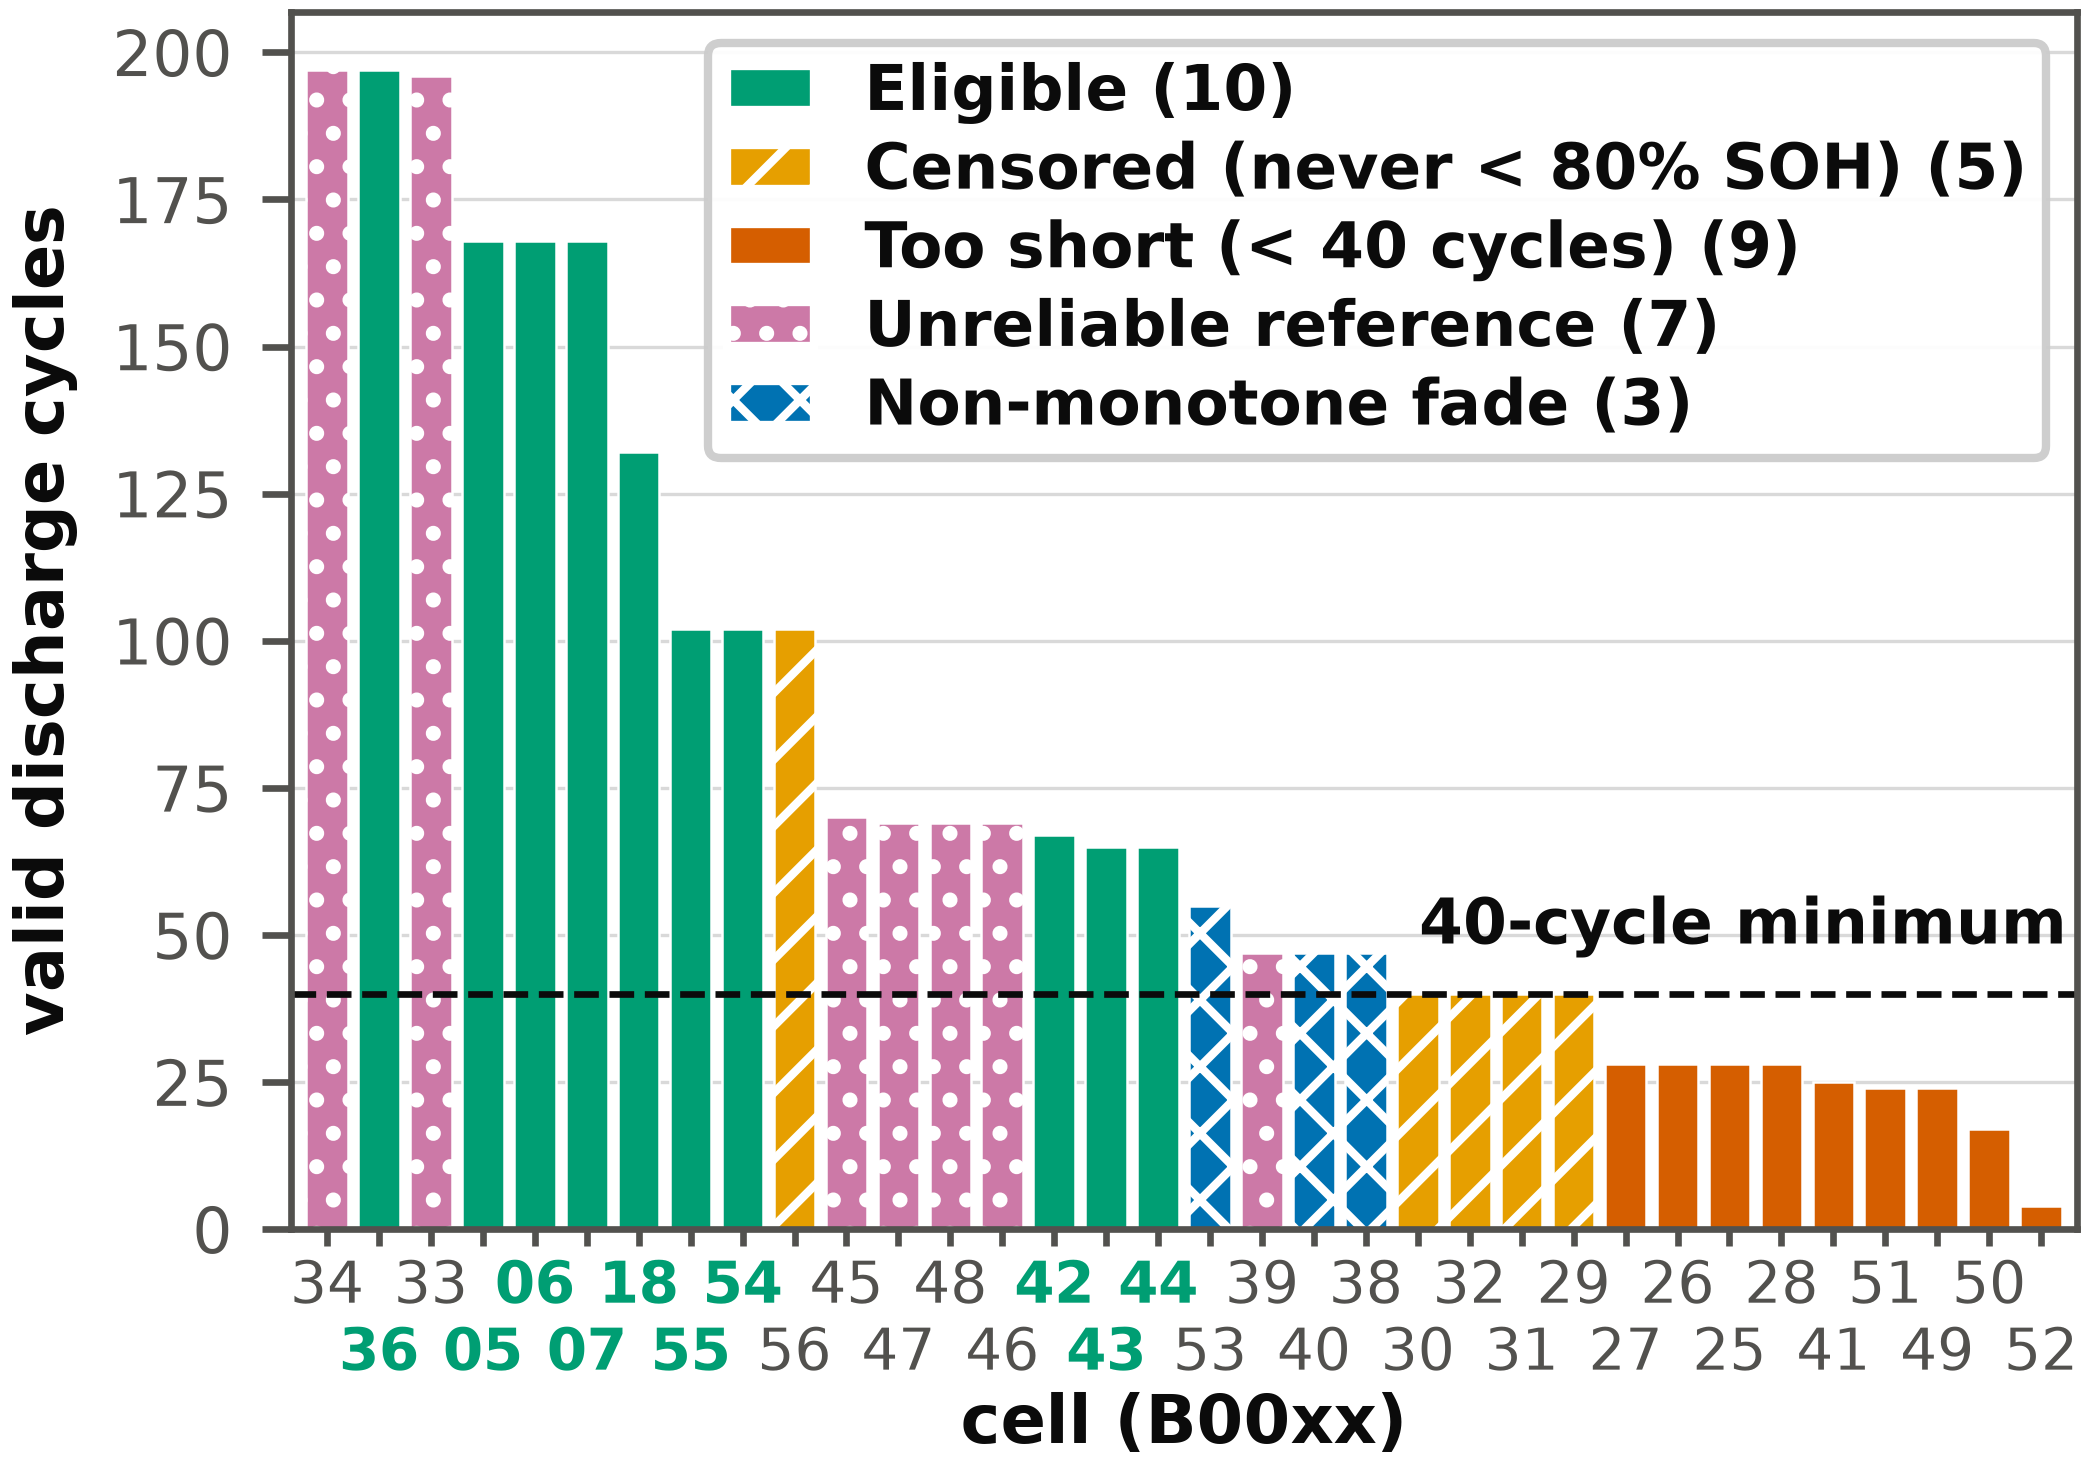
\includegraphics[width=0.76\columnwidth]{figs/fig1_screening.png}
\caption{Screening outcome for all 34 PCoE cells: cycle count per cell,
coloured by outcome, with the 40-cycle minimum; legend entries give the
category totals.}
\label{fig:screen}
\end{figure}

\subsection{Features and labels}
$Q_{\mathrm{ref}}$ is estimated once from an early-life window; since all
reported predictions are taken at $\lambda \geq 0.5$, beyond that window, the
feature set is causal (computable online at cycle $k$) at every evaluated
horizon: the current and ten
lagged smoothed-SOH values; rolling fade slopes over 10 and 25 cycles;
rolling 10-cycle SOH standard deviation; a cumulative capacity-regeneration
count; $Q_{\mathrm{ref}}$; ambient temperature; and forward-filled $R_e$ and
$R_{ct}$ (19 features in total, median-imputed where impedance is absent).
They cover what a BMS observes online: fade level, slope and noise, operating
condition and cell quality, and resistance growth; the SOH lags are nearly
collinear (Spearman $\rho\geq0.89$, Fig.~\ref{fig:corr}). Impedance is
missing only for 8--18\% of the cycles of B0005--B0007, but test counts differ
by campaign (278 versus 48--92), so Section~V-F ablates it. Per model, an
inner leave-one-cell-out loop over each fold's nine training cells selects
whether to add the cycle age $k$ and to predict $\mathrm{RUL}_k/k$; the
held-out cell never enters this choice. The label is $\mathrm{RUL}_k = k_{\mathrm{EOL}} - k$ for $k \leq
k_{\mathrm{EOL}}$, giving 735 labeled cycles across the cohort.

\begin{figure}[!t]
\centering
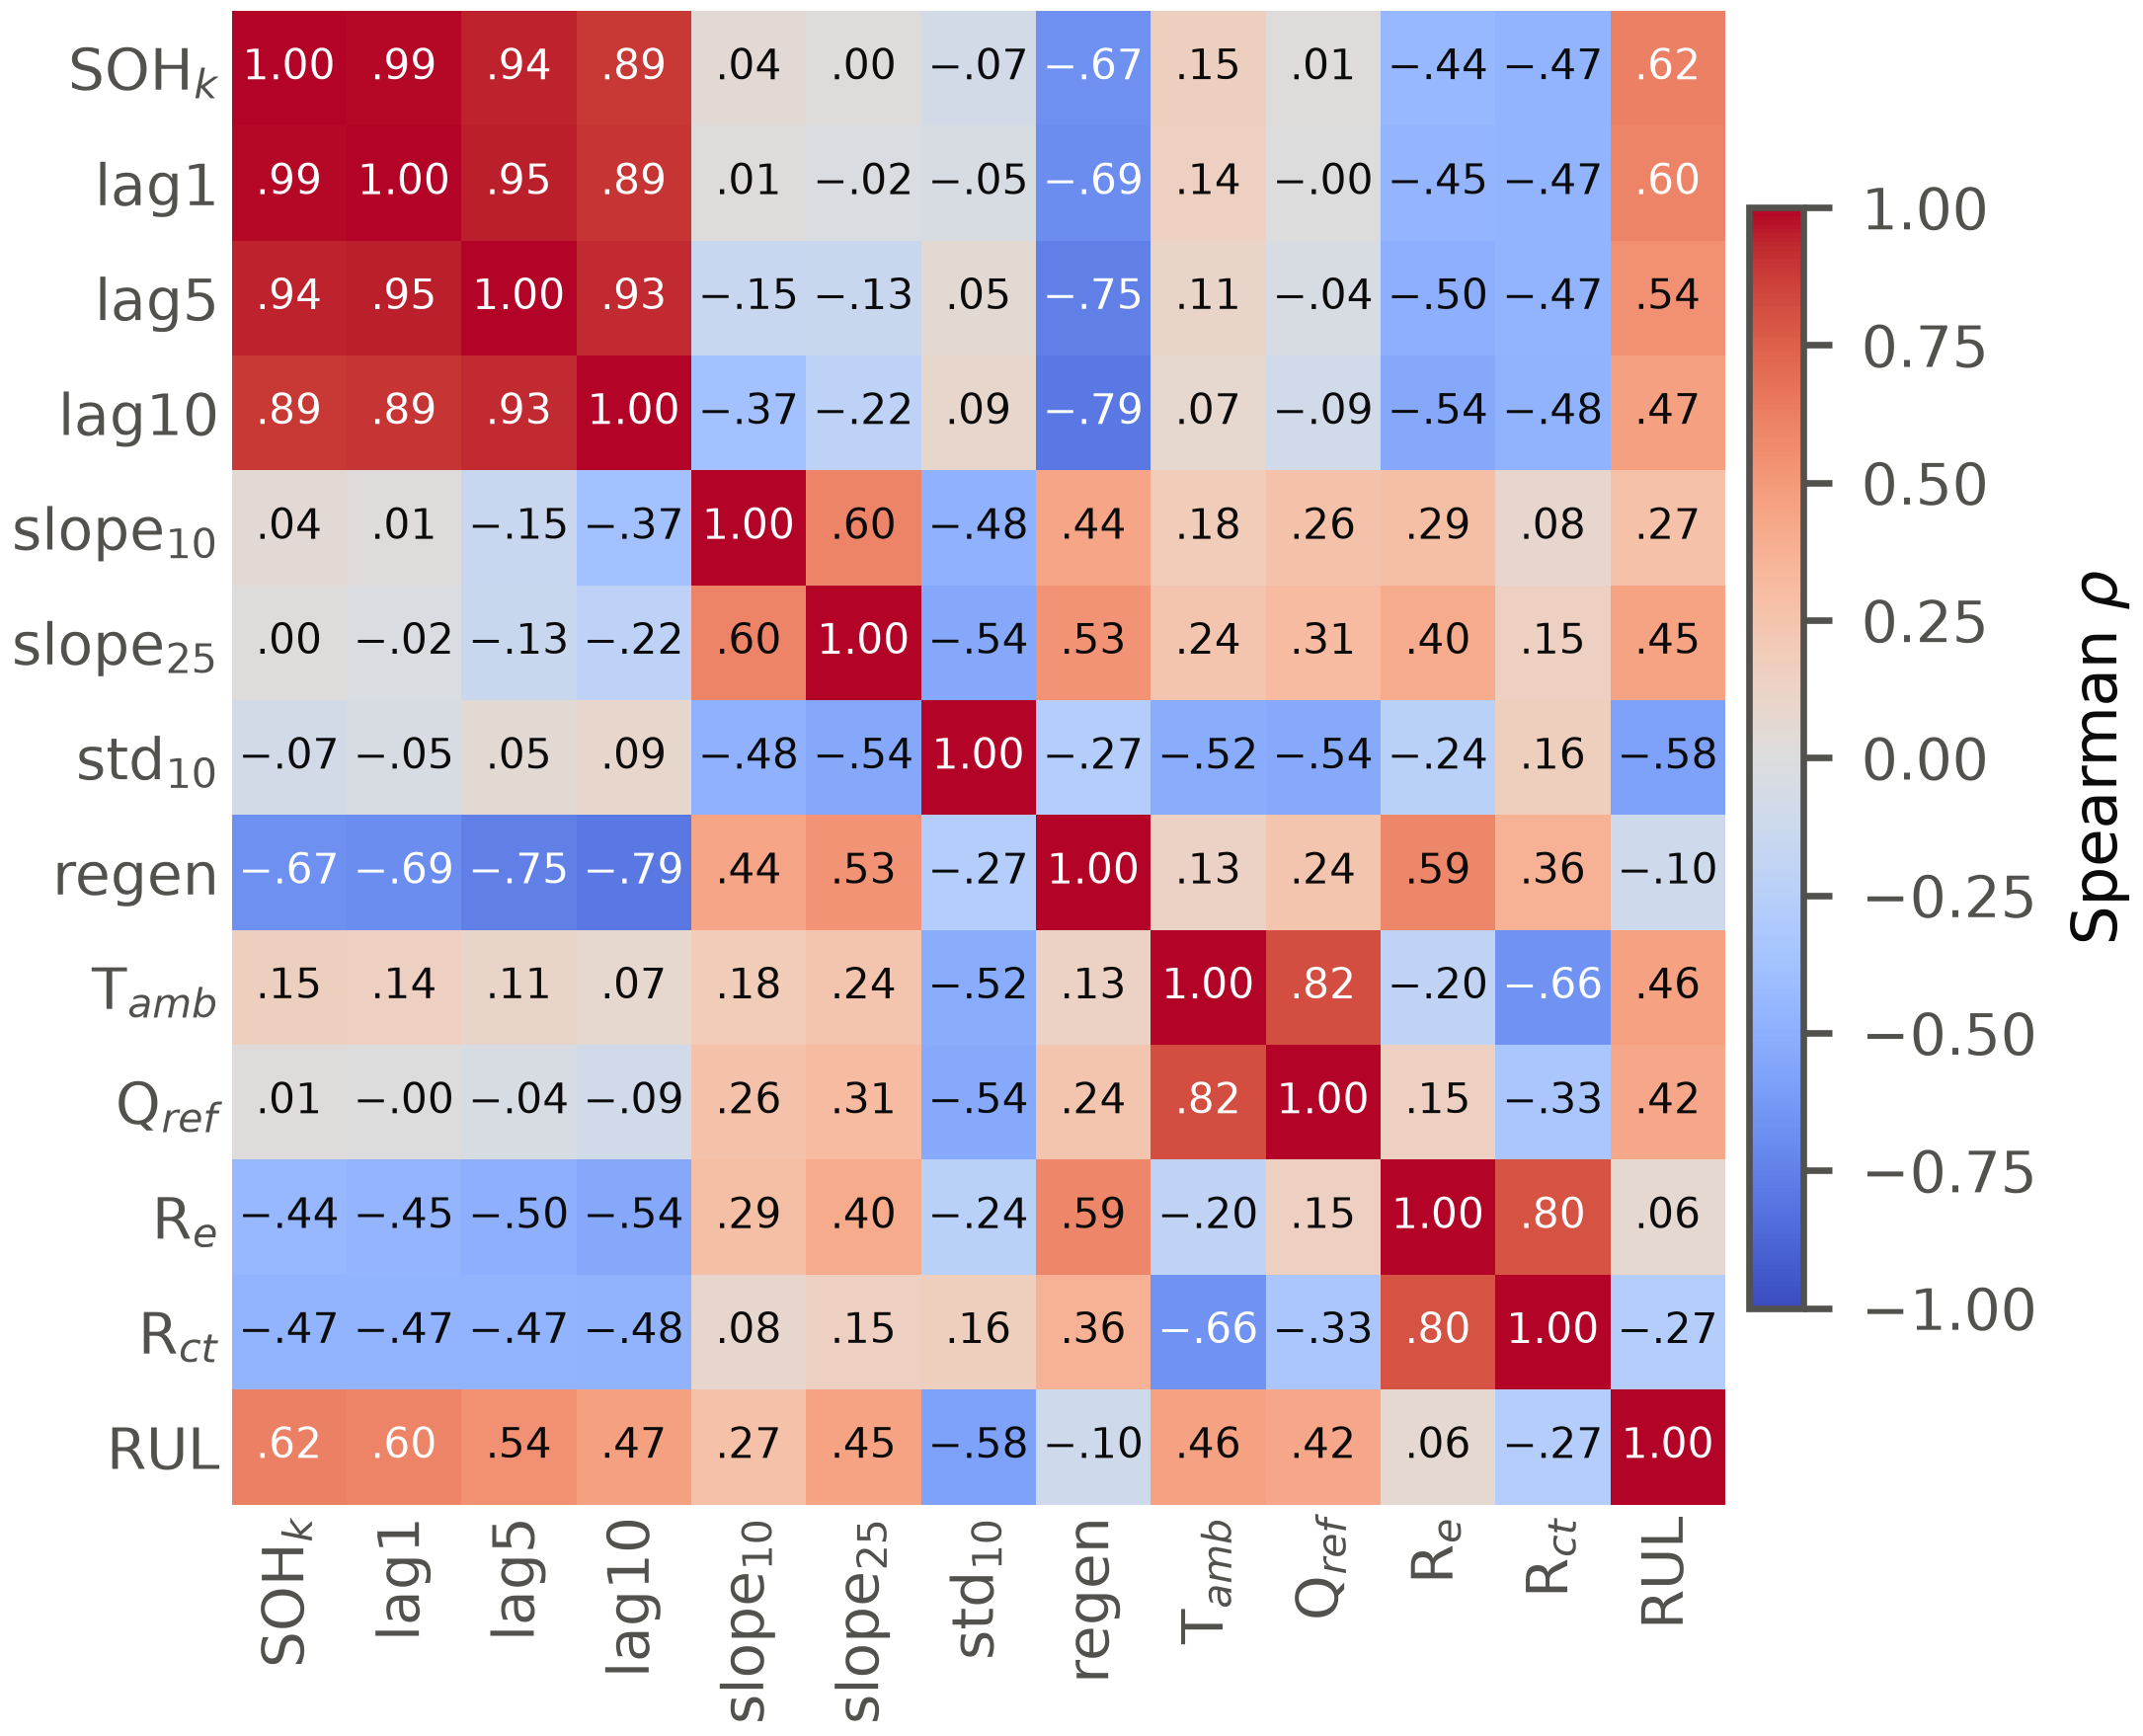
\includegraphics[width=0.8\columnwidth]{figs/fig_corr.png}
\caption{Spearman correlation of the RUL features and the label (SOH lags
2--4, 6--9 omitted; all lags have $\rho\geq0.89$).}
\label{fig:corr}
\end{figure}

\subsection{Evaluation protocol}
\textbf{LOBO.} For each of the ten folds, one cell is held out entirely; all
models are trained on the remaining nine.
\textbf{Same-cell control.} To quantify leakage, the identical models are
trained on the first 60\% of each cell's own life and tested on the
remainder---the protocol that dominates the literature. Its test segment
starts at $0.6\,k_{\mathrm{EOL}}$, so $\lambda=0.5$ is not scored and all
same-cell figures are out-of-sample; a \emph{matched} variant adds the nine
other cells to its training set, holding training size nearly constant.
\textbf{Metrics.} At life fractions $\lambda \in \{0.5, 0.7, 0.9\}$ we report
MAE and RMSE of predicted RUL across cells, the EOL hit rate
$|\hat{k}_{\mathrm{EOL}} - k_{\mathrm{EOL}}| \leq 10$ cycles and
$\alpha$--$\lambda$ accuracy with $\alpha = 0.2$~\cite{saxena2008}. Because
each fold contributes one error per cell, we also report the standard
deviation of the per-cell absolute error, bootstrap (over cells) 95\% CIs,
and test model pairs with a paired Wilcoxon signed-rank test.

\subsection{SOC track: data, label and features}
The RUL track above uses one aggregate per cycle. The SOC track instead needs
the within-cycle waveform, so we additionally process 164 complete discharge
records---a systematic every-fifth-cycle sample of six cells spanning all
three temperatures (B0005--B0007, B0018 at 24\,$^\circ$C; B0042 at
22\,$^\circ$C; B0054 at 4\,$^\circ$C)---giving \textbf{47{,}144} labelled
time steps of measured voltage, current and temperature.

\textbf{A non-tautological reference label.} SOC is coulomb-counted and
referenced to the cell's early-life capacity $Q_{\mathrm{ref}}$, not to the
capacity of the cycle being labelled:
\begin{equation}
\mathrm{SOC}(t) = 100 \cdot \frac{C_k - \int_0^{t} |I(\tau)|\,d\tau}{Q_{\mathrm{ref}}} .
\end{equation}
Normalizing by each cycle's own capacity---the common shortcut---would force
every cycle to start at exactly 100\% and thereby bake the aging state into
the label. With~(1) a fresh cycle starts near 100\% and an aged one starts
near its SOH which is the physically correct statement that an aged cell
simply holds less usable charge.

\textbf{Features} are causal except the cycle's SOH, known only after
discharge (removed in Section~V-D): instantaneous $V$, $I$, $T$; their
time derivatives $dV/dt$, $dT/dt$; 10-sample rolling means of $V$ and $T$;
charge removed so far; instantaneous power; ambient temperature; and the
cycle's SOH. \textbf{Baseline.} An open-circuit-voltage (OCV) lookup fitted
on the \emph{first} cycle of the training cells only provides a genuine
physics reference: unlike coulomb counting it never sees the label
construction. It is deliberately a single-signal reference and is not
feature-matched to the learned models, so it bounds what voltage alone
can supply rather than serving as a like-for-like competitor. Coulomb
counting with \emph{estimated} capacity adds two references: rated 2\,Ah
throughout (CC-nominal) and the previous cycle's capacity $C_{k-1}$ for $C_k$
(CC-prev).

\section{Methods}
\subsection{Model zoo}
Six models are benchmarked with identical features: ordinary
least squares and ridge regression (linear baselines), random forest,
XGBoost~\cite{chen2016}, LightGBM~\cite{ke2017} and \emph{lite-TFT} a
from-scratch temporal fusion transformer variant~\cite{lim2021} comprising a
gated-residual-network (GRN) variable-selection block with a weight-tied
per-feature transform, an LSTM encoder, multi-head self-attention and a GRN
output head (20{,}173 parameters), trained on 10-cycle sequences with Huber
loss, dropout 0.1, weight decay $10^{-5}$ and early stopping on one training
cell per fold (patience 12, $\leq$120 epochs), which cuts its per-cell spread
from $\pm$32.7 (fixed 60 epochs) to $\pm$13.1 cycles. Hyperparameters are fixed
defaults (ridge $\alpha=1$; 300 forest trees; 400 boosted trees of depth 4,
rate 0.05), never tuned on held-out cells. Its variable-selection weights are retained for
interpretability.

\subsection{Split conformal prediction}
For each LOBO fold, two of the nine training cells are held out as a
calibration set. A model $\hat{f}$ is fit on the remaining seven cells and
the conformity scores $s_i = |y_i - \hat{f}(x_i)|$ are computed on the
calibration cells. With $n$ calibration points, the interval half-width is
the $\lceil (n+1)(1-\alpha_c) \rceil / n$ empirical quantile $\hat{q}$ of the
scores at miscoverage $\alpha_c = 0.1$ and the prediction interval for a
test cycle is $\hat{f}(x) \pm \hat{q}$~\cite{lei2018}. Split conformal
guarantees $\geq 90\%$ marginal coverage \emph{under exchangeability};
holding out whole cells for calibration deliberately preserves the cross-cell
distribution shift, so any coverage shortfall directly measures how far the
deployment setting departs from that assumption. Because two cells give
noisy quantiles, we also report cell-grouped CV+~\cite{barber2021}, leaving
each training cell out once, with coverage pooled and per $\lambda$.

\subsection{Deployability measurement}
Each trained model is serialized to obtain its memory footprint and
single-thread CPU inference latency is measured per cycle-prediction. The
lite-TFT footprint is computed from its parameter count at float32. Trees are
also sized as C arrays in flash and lite-TFT RAM as its summed activations. These
figures are read against ESP32-class constraints ($\sim$520\,kB SRAM,
4--16\,MB flash), a representative low-cost BMS platform.

\section{Results and Discussion}
\begin{figure}[!htbp]
\centering
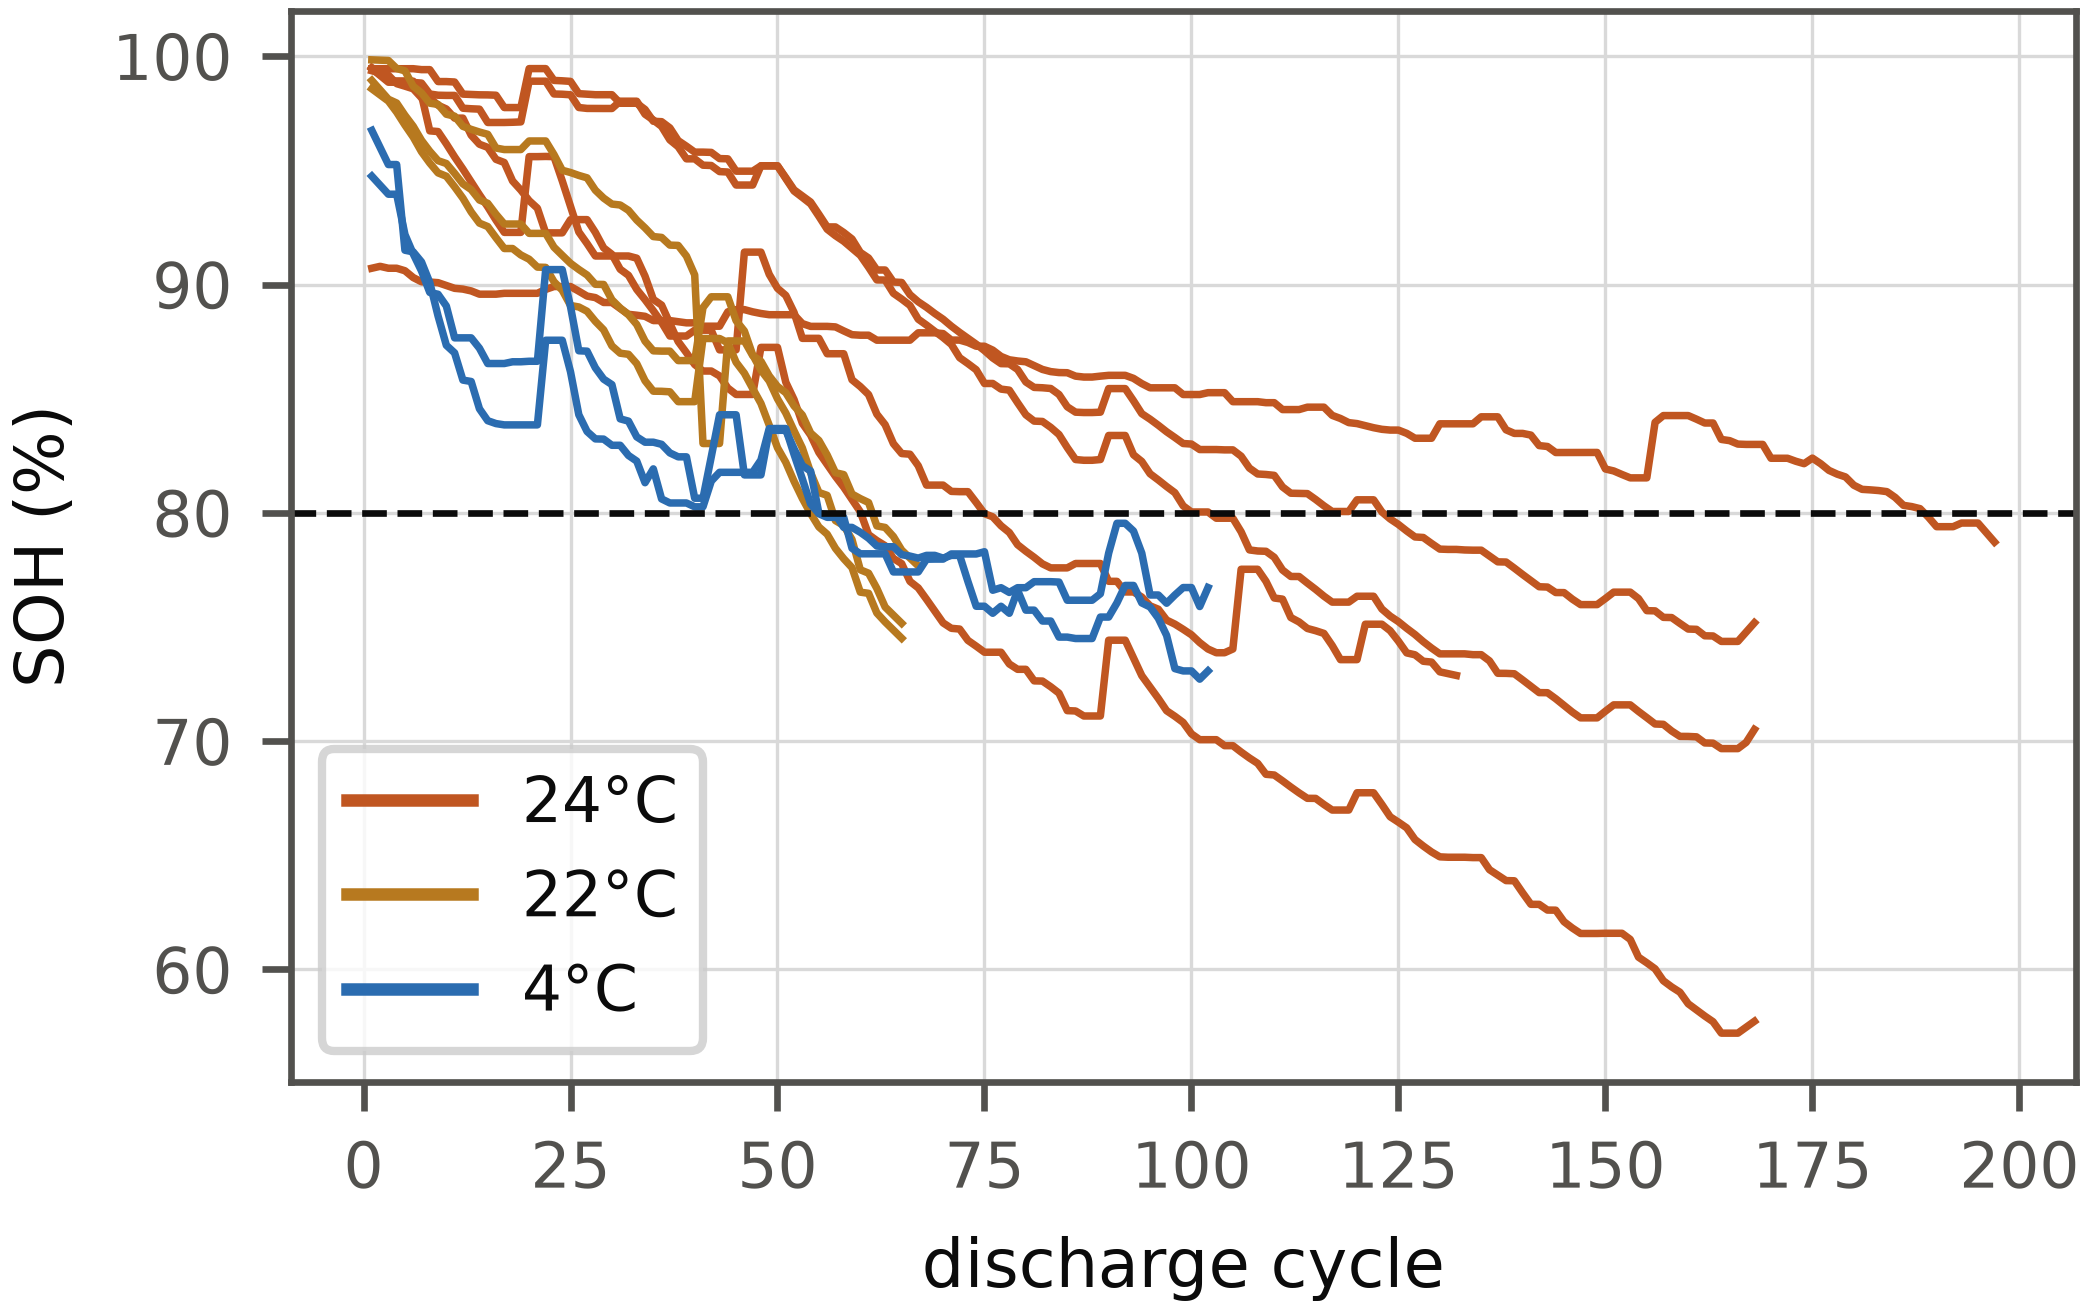
\includegraphics[width=0.66\columnwidth]{figs/fig2_cohort_soh.png}
\caption{Smoothed SOH trajectories of the 10-cell benchmark cohort, colored
by ambient temperature. The dashed line marks the 80\% SOH EOL threshold.}
\label{fig:cohort}
\end{figure}

\begin{table}[!htbp]
\caption{LOBO benchmark at 80\% SOH EOL (10 folds). MAE/RMSE in cycles;
MAE @ 0.7 is given as mean $\pm$ standard deviation across the ten held-out
cells (95\% CIs about $\pm$7). HR = EOL hit rate $\pm 10$ cycles and $\alpha$-acc at $\lambda=0.7$.}
\label{tab:lobo}
\centering
\small
\setlength{\tabcolsep}{3pt}
\begin{tabular}{lccccccc}
\toprule
 & \multicolumn{3}{c}{MAE @ $\lambda$} & RMSE & & \\
\cmidrule(lr){2-4}
Model & 0.5 & 0.7 (mean $\pm$ sd) & 0.9 & @0.7 & HR & $\alpha$-acc \\
\midrule
RandomForest & 17.8 & \textbf{9.4} $\pm$ 12.6 & \textbf{4.1} & 15.2 & \textbf{0.7} & \textbf{0.5} \\
XGBoost      & \textbf{15.6} & 9.6 $\pm$ 11.2 & 8.5 & \textbf{14.3} & 0.6 & \textbf{0.5} \\
LightGBM     & 20.2 & 12.2 $\pm$ 10.6 & 5.9 & 15.8 & 0.6 & 0.2 \\
Ridge        & 25.0 & 12.4 $\pm$ 8.8 & 17.0 & 14.9 & 0.5 & 0.2 \\
Linear       & 28.7 & 21.2 $\pm$ 18.4 & 15.3 & 27.5 & 0.3 & 0.1 \\
lite-TFT     & 19.0 & 13.2 $\pm$ 13.1 & 14.5 & 18.2 & 0.6 & 0.3 \\
\bottomrule
\end{tabular}
\end{table}

\subsection{Cross-cell benchmark}
Table~\ref{tab:lobo} and Fig.~\ref{fig:models} report the LOBO results. The tree ensembles are
ahead of the linear baselines---random forest attains 9.4-cycle MAE at 70\% of
life, improving to 4.1 cycles at 90\%, against 21.2 for ordinary least
squares ($p\leq0.014$) and 12.4 for ridge ($p\geq0.38$)---but they are \emph{not} separable from one another: the per-cell
standard deviation ($\pm$10.6 to $\pm$12.6 cycles) matches the mean in
magnitude and paired Wilcoxon tests return $p=0.23$ for random forest versus
XGBoost and $p=0.06$ for XGBoost versus LightGBM. Differences of one to two cycles
which the same-cell literature presents as improvements are inside the noise
at this cohort size. One fold dominates the spread: B0036, the longest-lived
cell at 197 cycles, is worst for five of six models (32.7 cycles for XGBoost
against 0.1 for B0042).

The lite-TFT trails on MAE (13.2 cycles; HR 0.6). With ten cells, HR and
$\alpha$--$\lambda$ accuracy move in steps of 0.1 (CIs $\pm$0.3), so they cannot
rank models at this cohort size.

\subsection{The leakage gap}
Fig.~\ref{fig:samecell} contrasts LOBO with the same-cell controls at
$\lambda=0.7$. Ridge regression which merely extrapolates the cell's own
nearly linear fade, achieves 3.1-cycle MAE same-cell versus 12.4 cycles under
LOBO. The best honest
error (9.4) is $\sim$3$\times$ the best leaky one (3.1). The matched control
attributes part of this to training-set size: given the nine other cells,
seeing the cell's own first 60\% lowers the best error from 9.4 to 6.0
cycles ($\sim$1.6$\times$). Notably, the tree
ensembles \emph{invert} at $\lambda = 0.9$ same-cell (MAE 35--42): trees
cannot extrapolate below the RUL range seen in training, whereas linear
models can---so the two protocols do not even preserve model rankings. Both
observations explain how the literature's near-perfect same-cell numbers
\cite{ceemdan2025,tlstm2025} coexist with collapsed cross-cell
performance~\cite{cnnframework2026} and argue that same-cell results should
only ever be reported alongside a cross-cell figure.

\begin{figure}[!t]
\centering
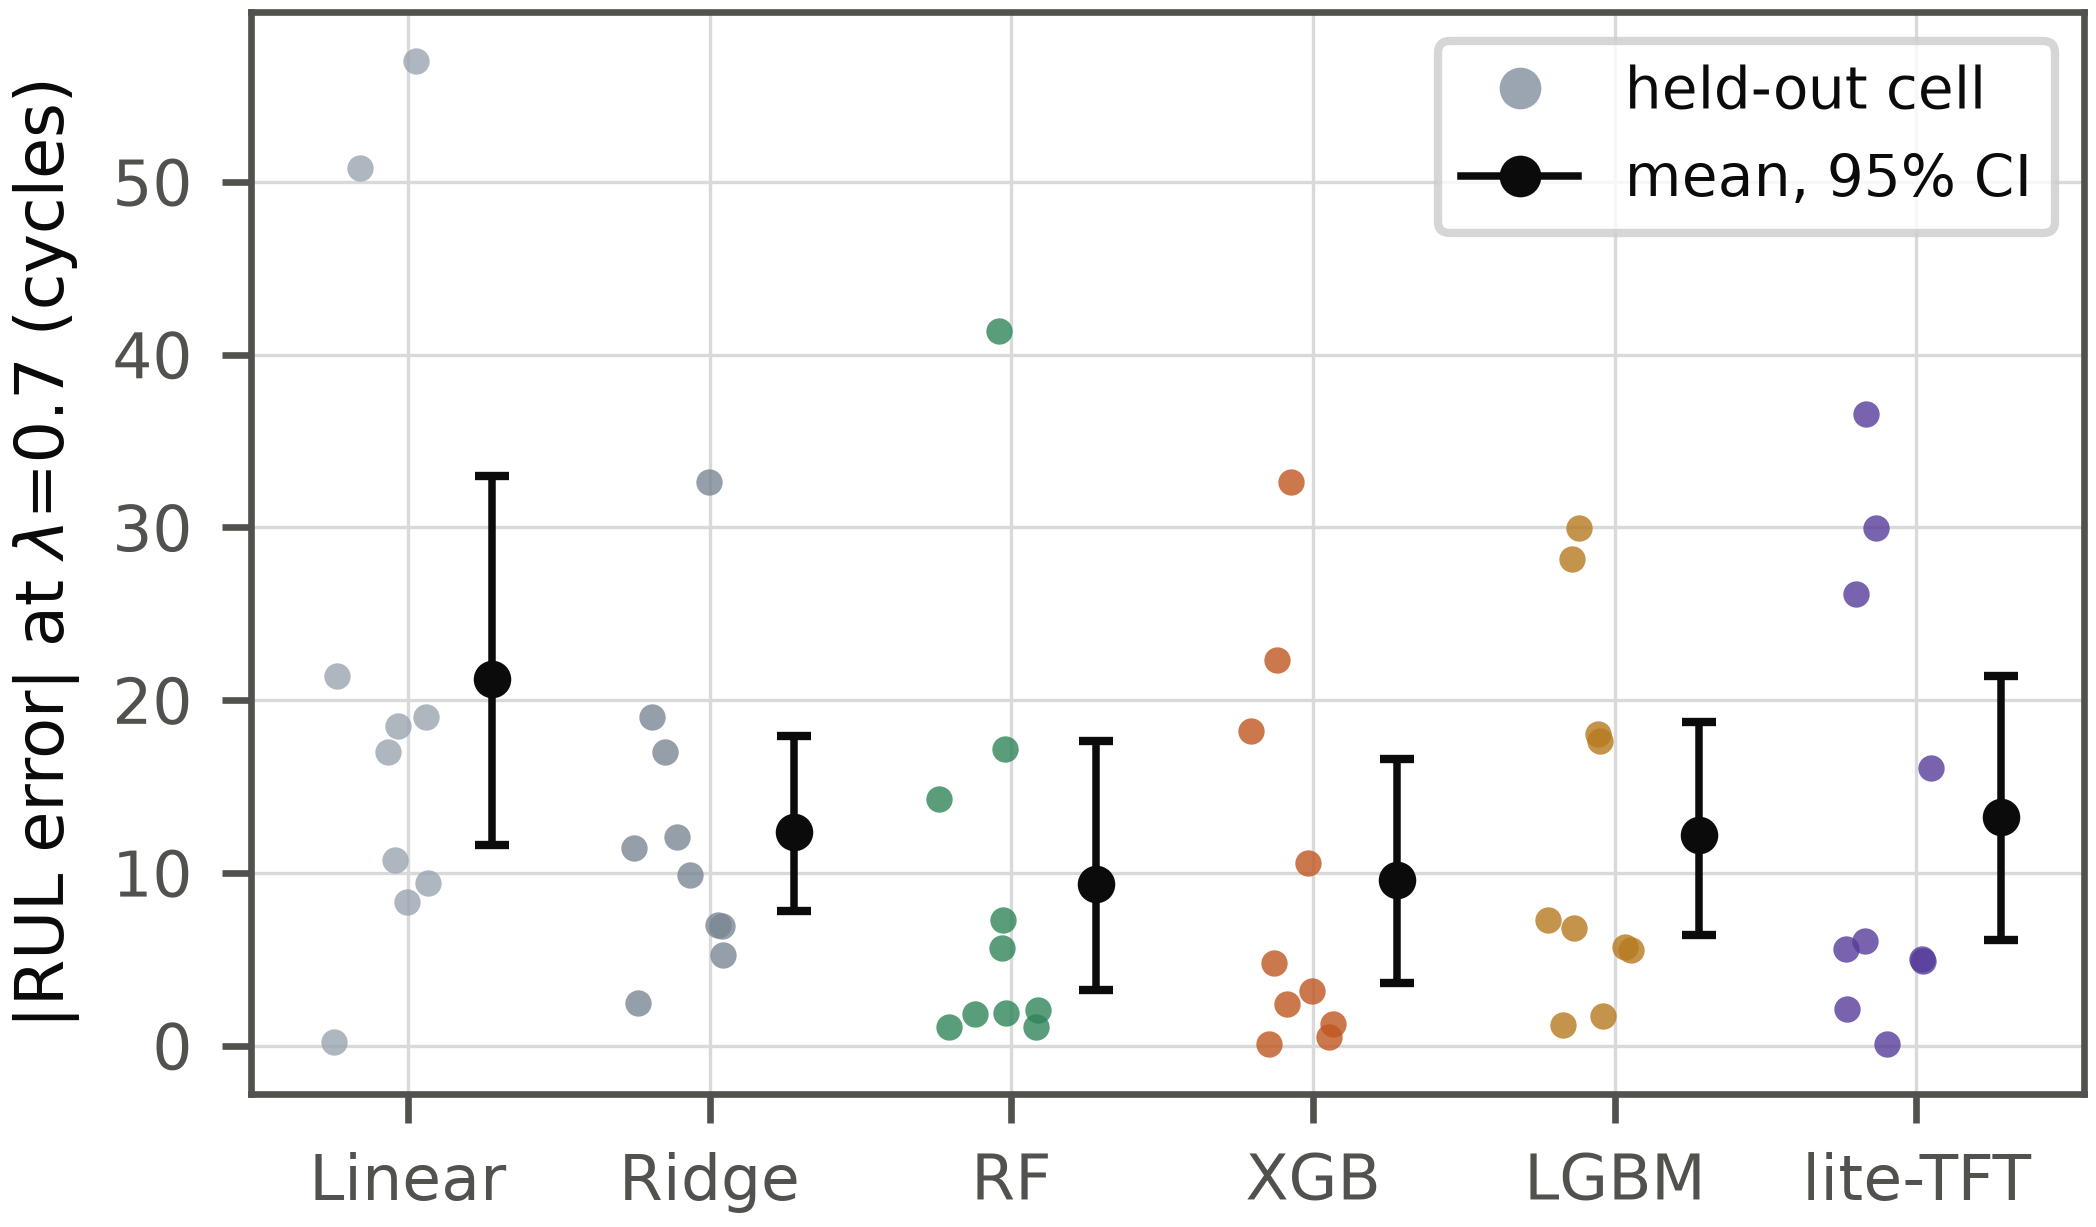
\includegraphics[width=0.8\columnwidth]{figs/fig3a_models.png}
\caption{LOBO RUL error at $\lambda=0.7$ for all six models, one dot per
held-out cell, with mean and bootstrap 95\% CI.}
\label{fig:models}
\end{figure}

\begin{figure}[!t]
\centering
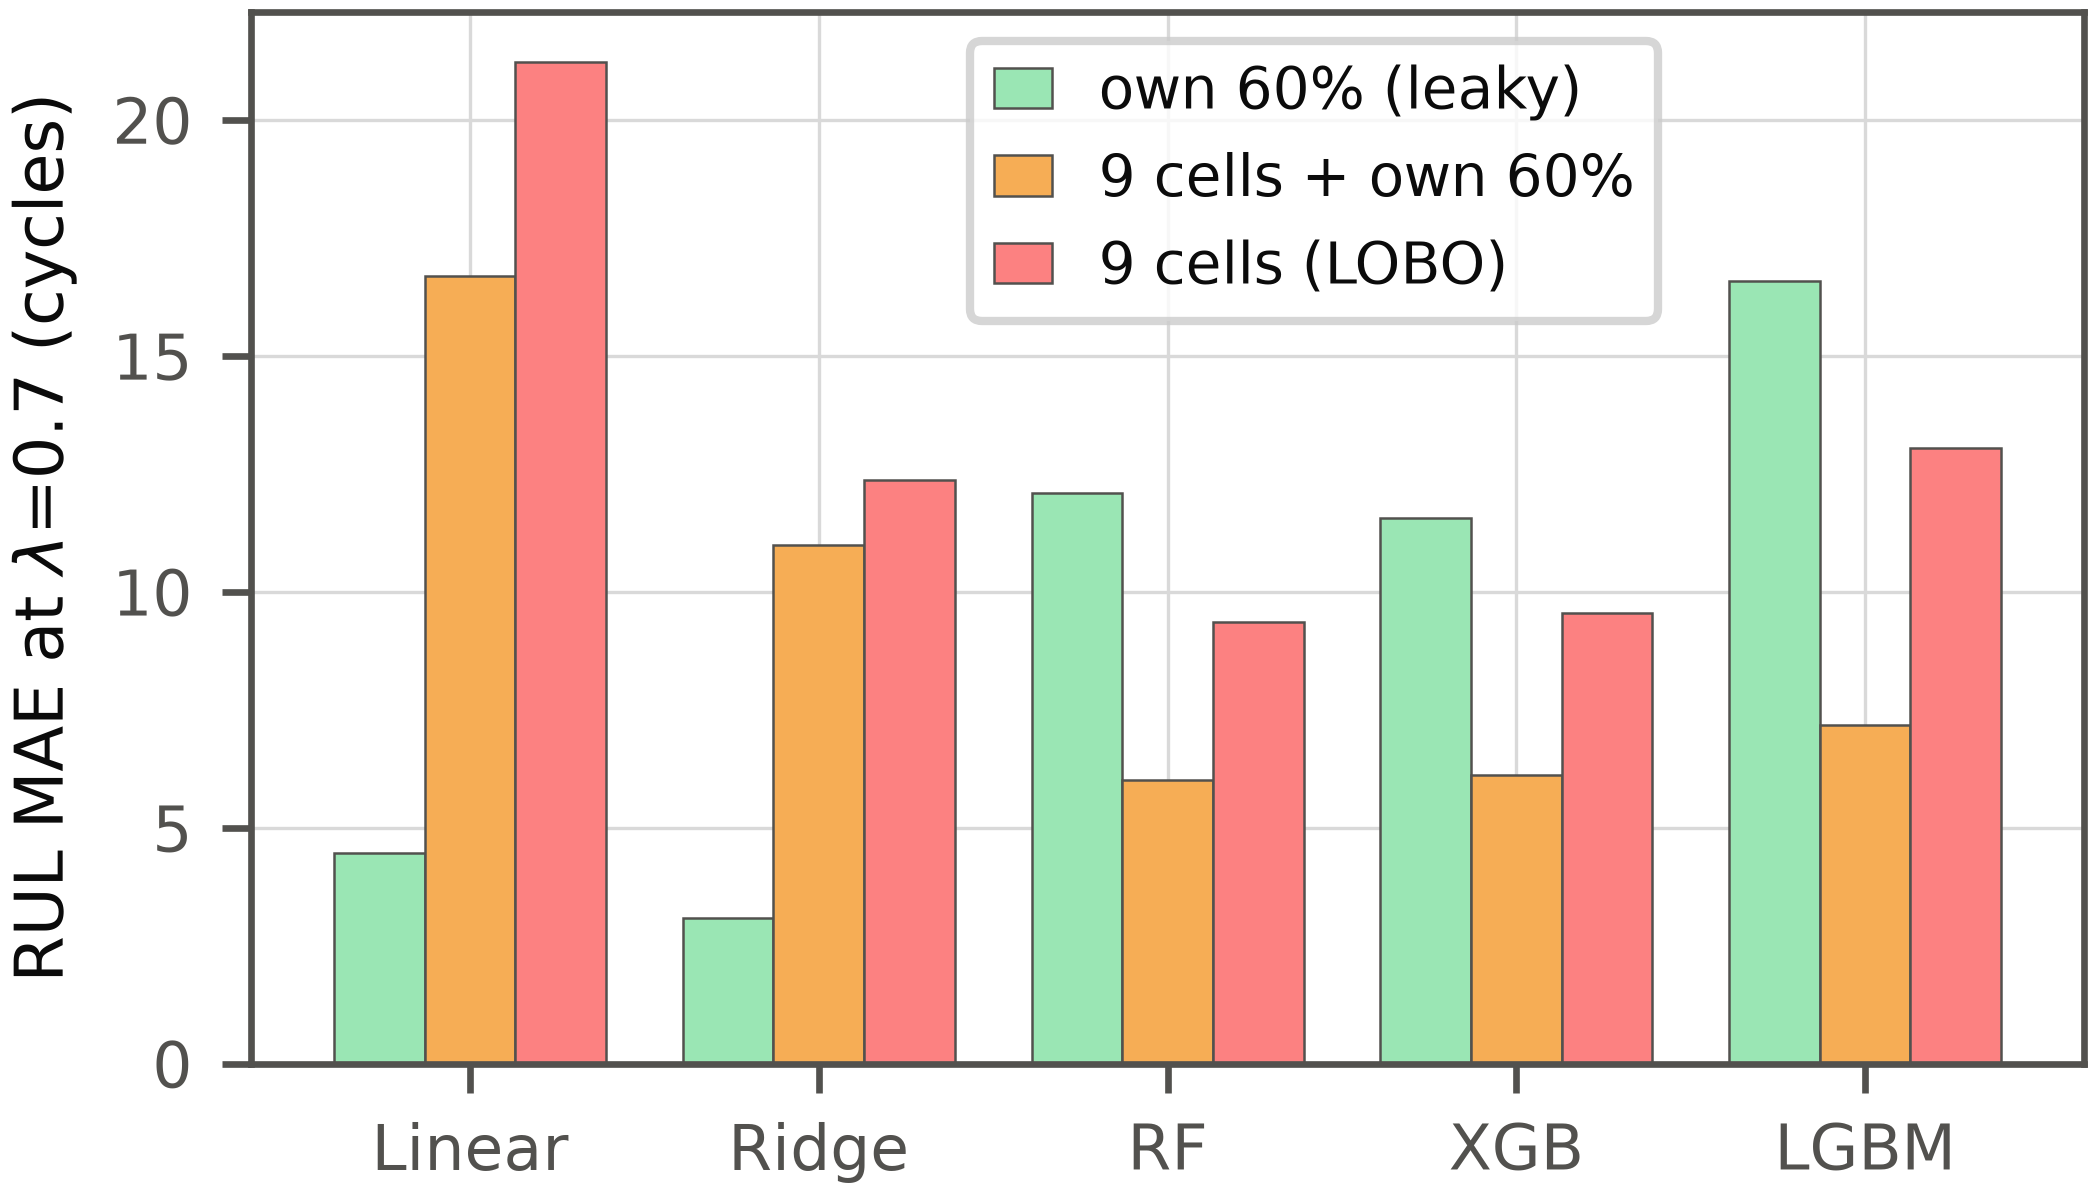
\includegraphics[width=0.8\columnwidth]{figs/fig3b_samecell.png}
\caption{Same-cell controls on identical test points: own first 60\%
(leaky), nine other cells plus own 60\% (matched) and nine cells only
(LOBO); the same models and features evaluated each way.}
\label{fig:samecell}
\end{figure}

\begin{figure}[!t]
\centering
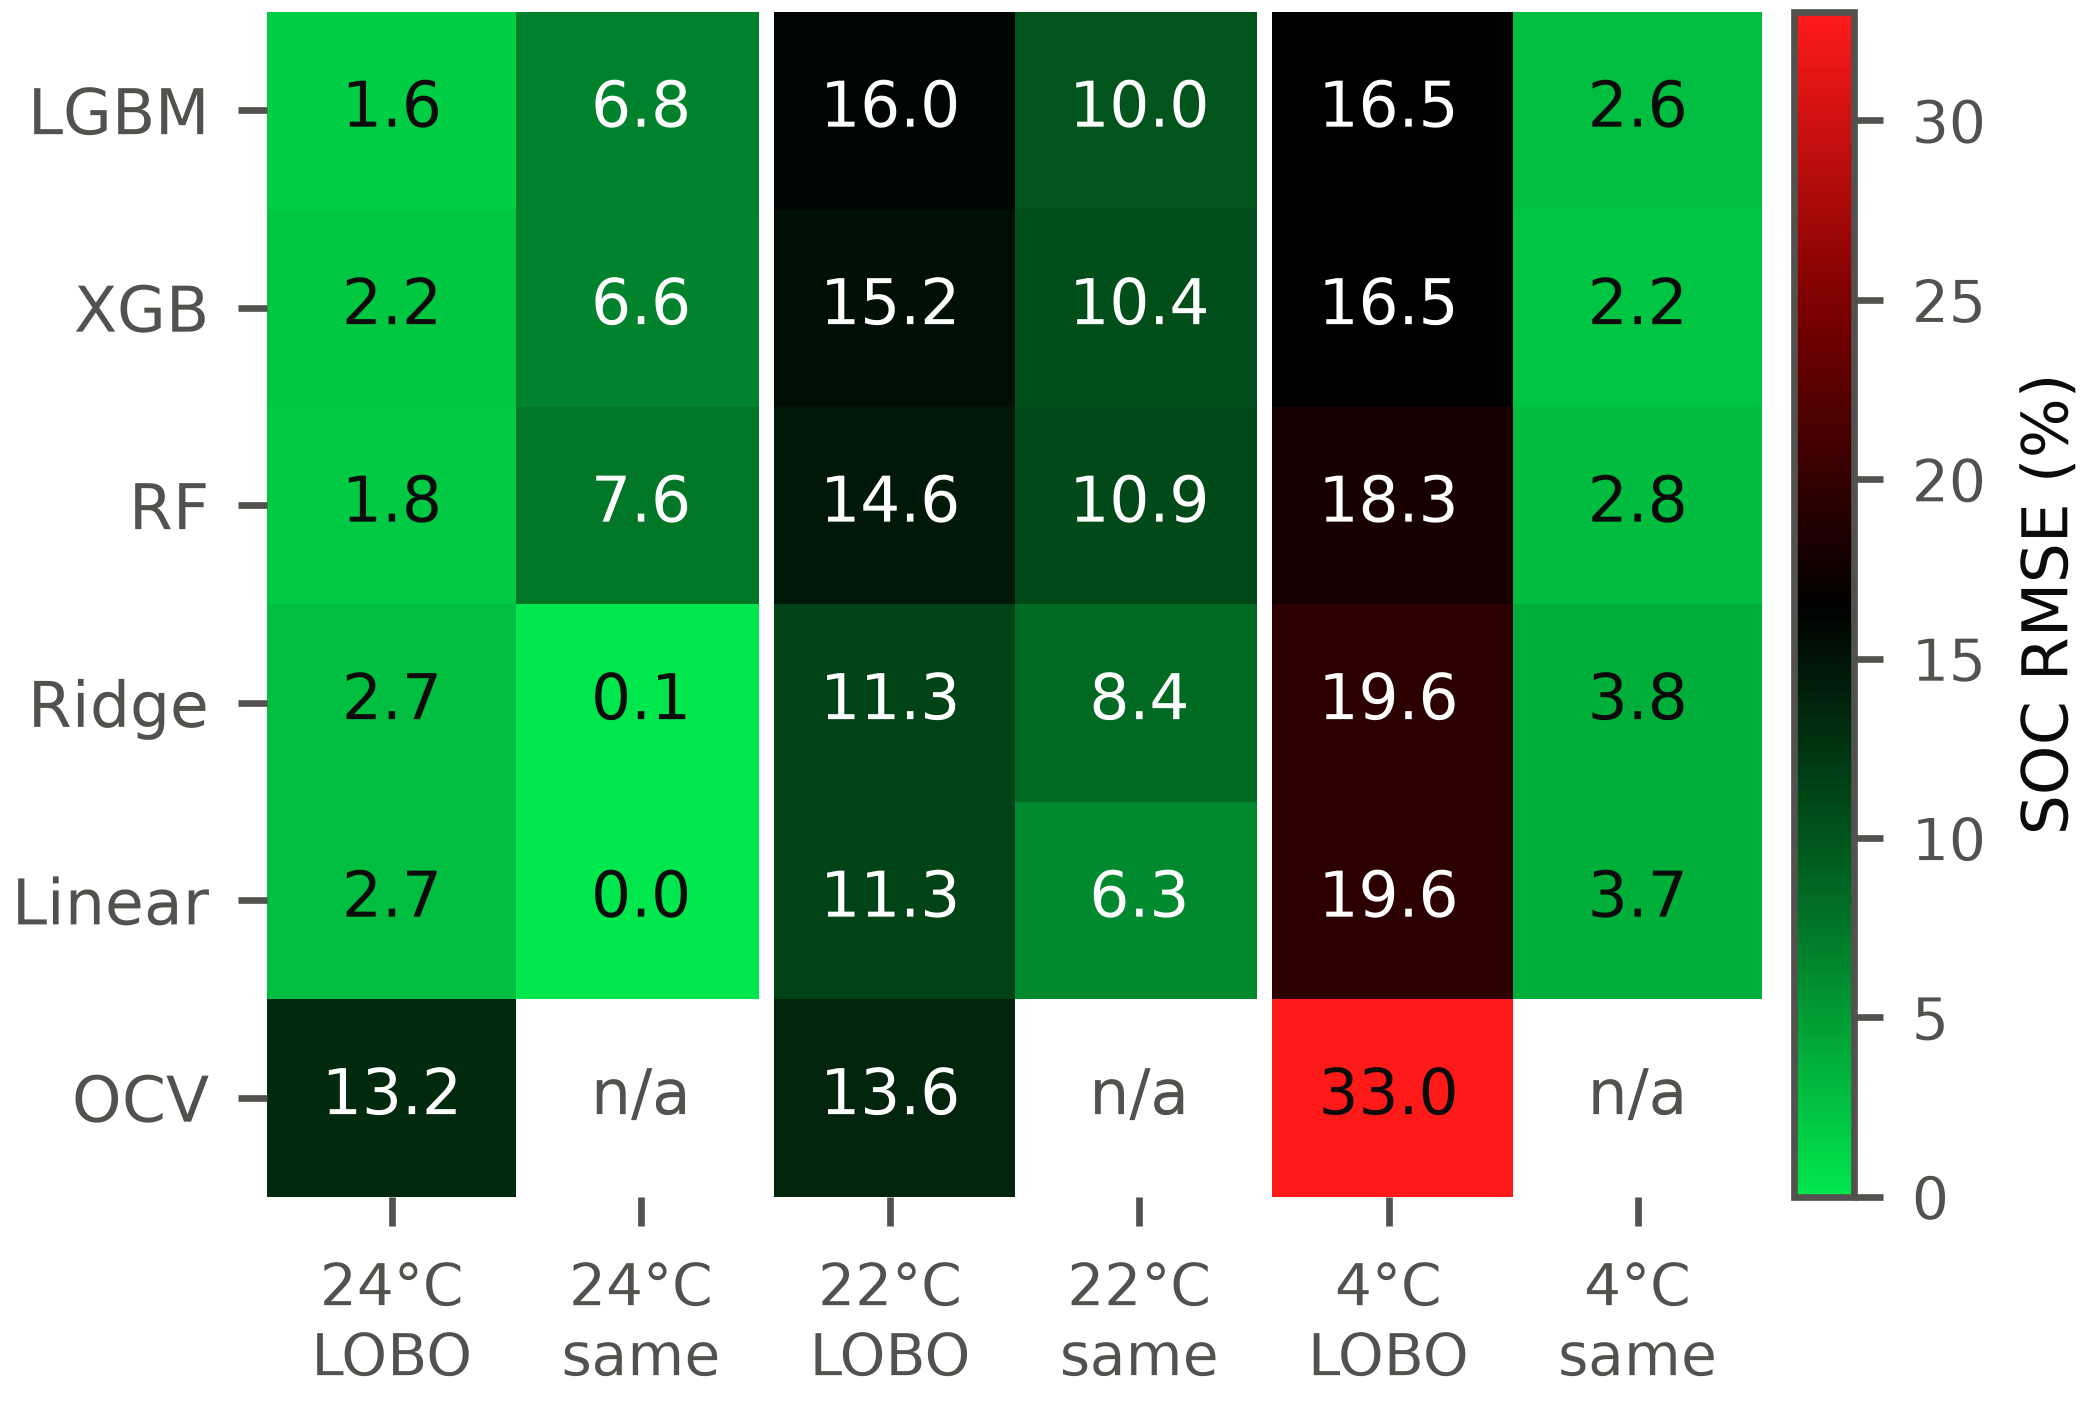
\includegraphics[width=0.8\columnwidth]{figs/fig4a_soc_heatmap.png}
\caption{SOC RMSE (\%) per model across ambient temperature $\times$
evaluation protocol; 47{,}144 held-out samples, 164 discharge cycles, 6
cells. The near-zero linear entries under 24\,$^\circ$C same-cell are the
algebraic artifact analysed in Section~V-D.}
\label{fig:soc}
\end{figure}

\begin{figure}[!t]
\centering
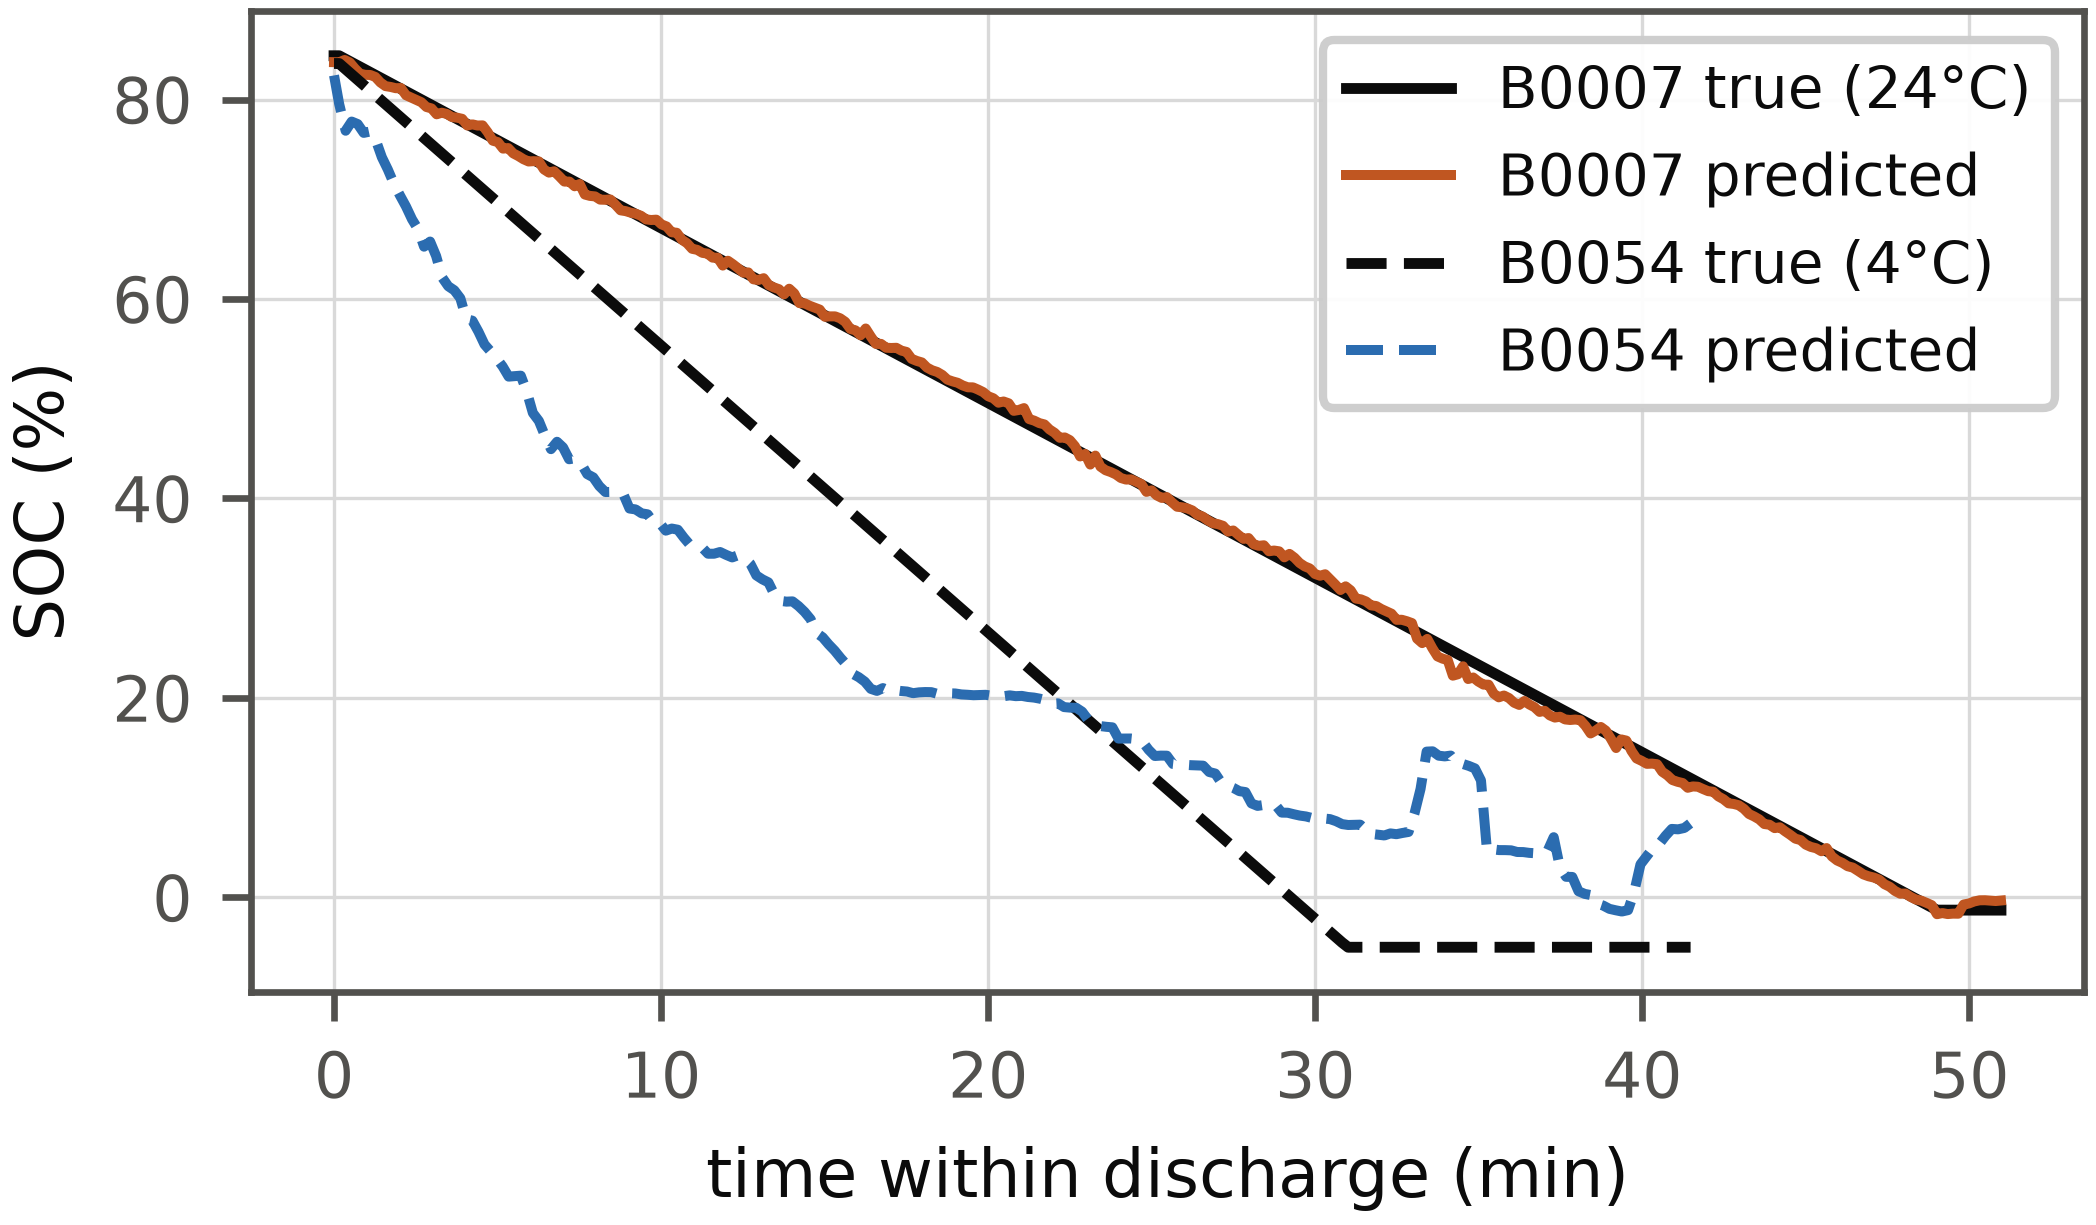
\includegraphics[width=0.72\columnwidth]{figs/fig4b_soc_traces.png}
\caption{Predicted versus true SOC (XGBoost) on a mid-life held-out cycle,
in-cohort (B0007, 24\,$^\circ$C) versus off-temperature (B0054,
4\,$^\circ$C).}
\label{fig:soctrace}
\end{figure}

\subsection{SOC: cells transfer within an operating group but not across it}
Fig.~\ref{fig:soc} reports the SOC track. Averaged over the six LOBO folds,
XGBoost attains 6.73\% RMSE and the OCV physics baseline 16.58\%---the
2.5$\times$ margin confirms the learned models add real information rather
than re-deriving the coulomb-counting identity which the label construction
was designed to prevent. The same-cell control again inflates accuracy: ridge
regression drops from 6.92\% RMSE under LOBO to 2.11\% when it may train on
the test cell and linear regression from 6.94\% to 1.67\%, a
$\sim$4$\times$ leakage gap that mirrors the RUL result of
Section~V-B.

The aggregate, however, hides the more useful finding. Splitting the folds
(Fig.~\ref{fig:soc}) shows that for the four cells held out from within the
24\,$^\circ$C group the error is 1.2--3.6\% RMSE---B0007 reaches
0.69\%---whereas the two cells drawn from outside it degrade to
13.7--18.1\%, a roughly sevenfold jump. Fig.~\ref{fig:soctrace} makes the failure
visible: on the 24\,$^\circ$C cell the predicted trace overlays the truth
almost exactly, while on the 4\,$^\circ$C cell it departs early and never
recovers the correct slope. \emph{Cell-to-cell variation within a homogeneous
group is therefore not the binding constraint on SOC estimation; leaving that
group is.}

We stop short of attributing this to temperature alone. Both out-of-group
cells (B0042 at 22\,$^\circ$C, B0054 at 4\,$^\circ$C) come from later PCoE
campaigns that also differ in discharge protocol and the evidence cannot
separate the factors: B0042 sits only 2\,$^\circ$C from the training
temperature yet degrades to 15.3\% RMSE under XGBoost which a two-degree
shift cannot explain. A SOC model validated within one operating group can
thus carry an order-of-magnitude larger error outside it---temperature
\emph{and} protocol are evaluation axes, not nuisance parameters.

\subsection{Why same-cell SOC evaluation is vacuous}
The Linear/Ridge entries in the 24\,$^\circ$C same-cell column of
Fig.~\ref{fig:soc} read 0.00 and 0.13\% RMSE. This is not estimation skill
and the reason generalizes. Expanding definition~(1) within a single cell,
\begin{equation}
\mathrm{SOC}(t) = \mathrm{SOH}_k - \frac{100}{Q_{\mathrm{ref}}}\int_0^t |I|\,d\tau ,
\end{equation}
so the label is an \emph{exact affine function} of two supplied features
(SOH and charge removed) whose slope $-100/Q_{\mathrm{ref}}$ is fixed for
that cell. A least-squares fit recovers the label definition algebraically
rather than learning anything: for B0005 it returns $(1.000, -53.87)$ with
zero maximum residual and $-100/(-53.87) = 1.856$\,Ah is exactly that cell's
$Q_{\mathrm{ref}}$. Across cells $Q_{\mathrm{ref}}$ changes, the slope
changes with it and no single affine map fits---which is why the honest LOBO
columns are two to seven times larger. Any SOC study reporting same-cell
error on a coulomb-counted label therefore risks reporting the identity it
started from; the cross-cell protocol is what makes the task real.

The same identity could explain the group effect, since $Q_{\mathrm{ref}}$
differs between groups (1.86--2.04\,Ah at 24\,$^\circ$C versus 1.73 and
1.17\,Ah). It does not: in-group/out-of-group RMSE is 2.4/14.4\% with the
causal $\mathrm{SOH}_{k-1}$, 4.6/15.3\% without SOH and 5.7/22.9\% without SOH
and charge removed. CC-nominal reaches 24.6\%, but CC-prev 2.6\%, below every
learned model; it differs from the label only in using $C_{k-1}$ for $C_k$,
so it reflects the label construction rather than estimation skill. The
learned models matter where integrated current or a capacity estimate is
unavailable---the last ablation.

\subsection{Calibrated uncertainty}
Split conformal intervals (Fig.~\ref{fig:cp}) achieve mean empirical coverage
of 0.75--0.83 against the nominal 90\% target (XGBoost 0.81, half-width 44
cycles) with large per-fold variance. The shortfall is not a defect of
conformal prediction but a measurement of the exchangeability violation:
calibration cells and the held-out cell come from visibly different
degradation distributions (Fig.~\ref{fig:cohort}). CV+ over all nine training cells
restores the target (0.91--0.93 pooled, $\geq$0.9 at each $\lambda$) but at
1.1 times a typical cell's life in half-width (XGBoost 78 cycles), and stays
bimodal: B0036, whose life exceeds the training range, reaches only 0.31.
Cell-conditional or normalized conformal methods are a natural next step.

\begin{figure}[!t]
\centering
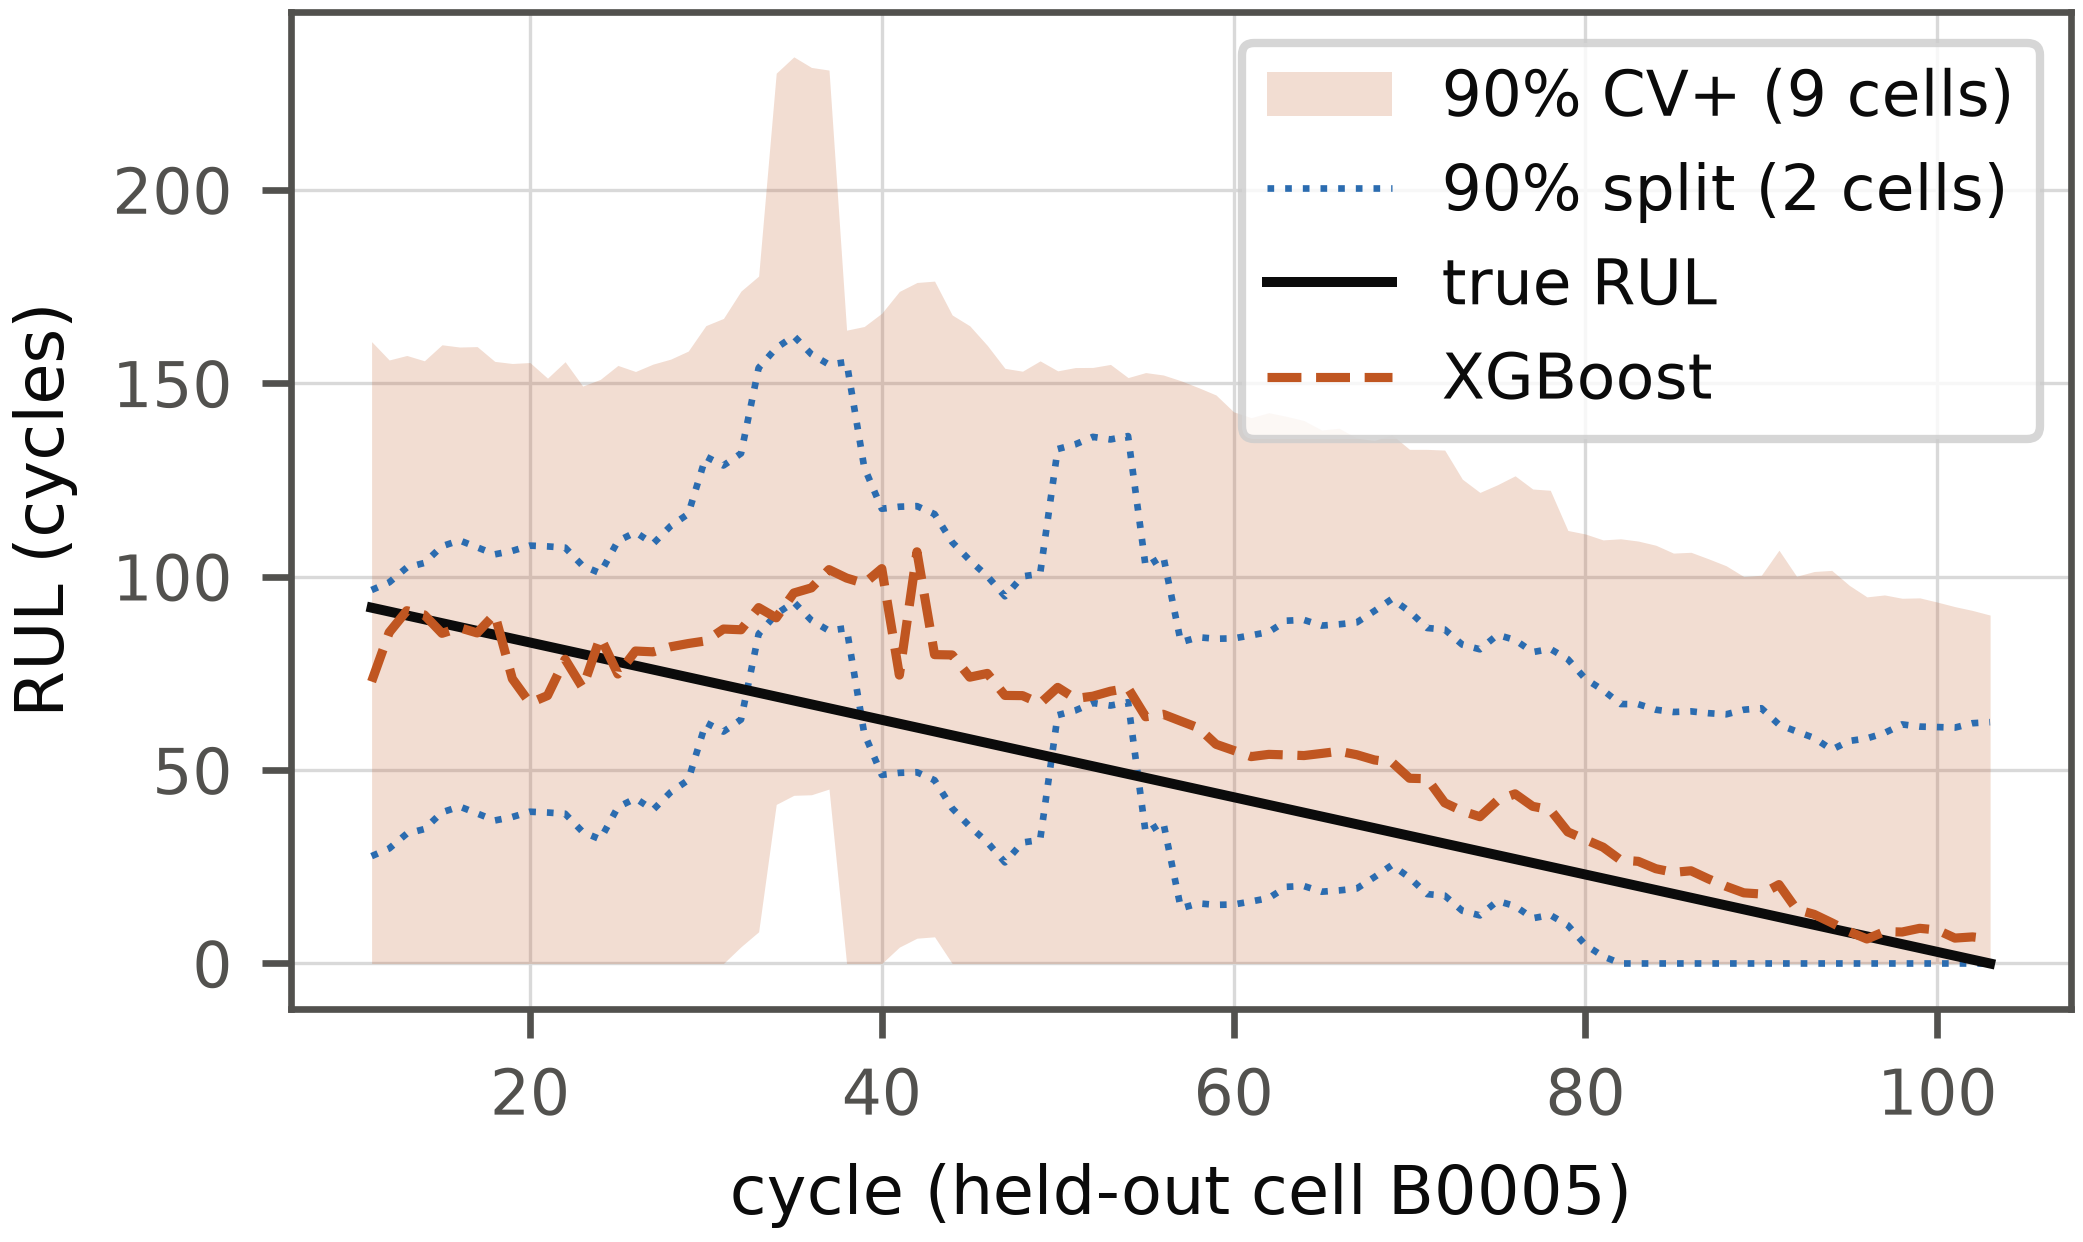
\includegraphics[width=0.68\columnwidth]{figs/fig5_conformal.png}
\caption{XGBoost RUL prediction with nominal 90\% CV+ band (shaded) and
split-conformal band (dotted) on held-out cell B0005 (never seen in training or calibration).}
\label{fig:cp}
\end{figure}

\subsection{Interpretability}
The lite-TFT's variable-selection weights, averaged over all folds, rank ambient
temperature first, then charge-transfer resistance $R_{ct}$, with
electrolyte resistance $R_e$ fourth---ahead of all but one SOH lag. This
is physically coherent, as temperature and impedance govern degradation
rate across cells. Since impedance availability follows the test campaign,
part of this weight may encode campaign identity: removing $R_e$ and $R_{ct}$
moves the tree ensembles by 0.9--1.6 cycles (within their CIs) but the
lite-TFT from 13.2 to 21.9 cycles.

\subsection{Edge deployability}
Table~\ref{tab:eff} shows that the accuracy leaders are also the compact
ones: XGBoost (400 trees of depth 4; 596\,kB, 6.8\,$\mu$s per prediction) and LightGBM
(328\,kB, 13.6\,$\mu$s) fit within ESP32 flash, ridge regression is
essentially free (0.6\,kB) and the lite-TFT's 20k parameters occupy 79\,kB
at float32 and 54\,kB under measured int8 quantization (biases and
normalization stay in floating point).
Only the random forest (19\,MB) is clearly edge-hostile. RAM, the binding
ESP32 constraint, is small: trees kept in flash need $<$0.2\,kB, and the
lite-TFT's activations total at most 185\,kB of 520\,kB.

These figures bound feasibility; they do not demonstrate deployment:
latency on a $\sim$240\,MHz core will be one to two orders of magnitude
higher. Tiny SOC networks have run on microcontrollers~\cite{pau2021},
\cite{warden2020}; measuring these models in situ is left to future work.

\begin{table}[!htbp]
\caption{Serialized size (C: C-array export) and desktop-CPU latency; last
column: footprint fits ESP32 flash (not an on-target test).}
\label{tab:eff}
\centering
\small
\begin{tabular}{lrrc}
\toprule
Model & Size (kB) & Latency ($\mu$s) & ESP32 flash \\
\midrule
Linear / Ridge & 0.8 / 0.6 & 0.8 / 0.8 & yes \\
XGBoost & 596 (62 C) & 6.8 & yes \\
LightGBM & 328 (37 C) & 13.6 & yes \\
lite-TFT & 79 (54 int8) & 1348 & yes \\
RandomForest & 19{,}062 (1{,}713 C) & 445 & no \\
\bottomrule
\end{tabular}
\end{table}

\subsection{Limitations}
The cohort is small (10 cells for RUL, 6 for SOC), the 4\,$^\circ$C
cells are under-represented and features are capacity/impedance histories
rather than full curves; one fold (B0036) dominates the spread. SOH is not
benchmarked as a prediction target, censored cells inform screening but not
training, and CV+ covers only with wide intervals. Only two SOC cells lie
outside the 24\,$^\circ$C group and they differ in both temperature and
protocol, so the sevenfold degradation is a direction for
\emph{out-of-group} transfer, not a temperature coefficient. The SOC label
is coulomb-counted, not a measured ground truth.

\section{Conclusion and Future Work}
This paper establishes an honest baseline for battery state estimation on the
full NASA PCoE corpus: a documented, censoring-aware screening; a
three-temperature LOBO benchmark covering RUL (10 cells) and SOC (6 cells)
leakage gaps of $\sim$3$\times$ (RUL) and
$\sim$4$\times$ (SOC) that reframe much of the same-cell state of the art
reported on PCoE; the finding that SOC transfers across
unseen \emph{cells} within one operating group but degrades roughly
sevenfold outside it, even without SOH features; and conformal intervals with honestly reported
under-coverage.

Future work: on-device deployment with int8 quantization; survival-analysis
training that exploits the censored cells; and richer within-cycle
features and cross-corpus transfer to CALCE and MIT/Stanford---which, by supplying cells
varying in temperature at fixed protocol, would separate the factors
confounded in Section~V-C.

\balance

\begin{thebibliography}{25}
\scriptsize
\setlength{\itemsep}{-1pt}
\setlength{\parskip}{0pt}

\bibitem{vidal2020} C. Vidal \emph{et al.},
``Machine learning applied to electrified vehicle battery state of charge
and state of health estimation: State-of-the-art,'' \emph{IEEE Access},
vol.~8, pp. 52796--52814, 2020.

\bibitem{doyle1993} M. Doyle, T. F. Fuller and J. Newman, ``Modeling of
galvanostatic charge and discharge of the lithium/polymer/insertion cell,''
\emph{J. Electrochem. Soc.}, vol.~140, no.~6, pp. 1526--1533, 1993.

\bibitem{santhanagopalan2006} S. Santhanagopalan \emph{et al.}, ``Review of models for predicting the cycling performance of
lithium ion batteries,'' \emph{J. Power Sources}, vol.~156, no.~2,
pp. 620--628, 2006.

\bibitem{saha2007} B. Saha and K. Goebel, ``Battery data set,'' NASA Ames
Prognostics Data Repository, NASA Ames Research Center, Moffett Field, CA,
2007.

\bibitem{ceemdan2025} Y. Fan \emph{et al.}, ``A hybrid
approach for lithium-ion battery remaining useful life prediction using
signal decomposition and machine learning,'' \emph{Sci. Rep.}, vol.~15,
no.~1, Art. no. 8161, 2025.

\bibitem{tlstm2025} S. Chen and X. Fang, ``Remaining useful life prediction
of lithium-ion batteries via spatial attention TLSTM and dilated CNN with
evolutionary optimization,'' \emph{Sci. Rep.}, vol.~15, no.~1,
Art. no. 32340, 2025.

\bibitem{cnnframework2026} M. Yenioglu, E. Aycicek and O. Erdinc, ``A
data-driven framework for lithium-ion battery remaining useful life
prediction using CNN and machine learning models,'' \emph{Batteries},
vol.~12, no.~4, Art. no. 135, 2026.

\bibitem{lei2018} J. Lei \emph{et al.}, ``Distribution-free predictive inference for regression,''
\emph{J. Amer. Statist. Assoc.}, vol.~113, no.~523, pp. 1094--1111, 2018.

\bibitem{tftenergy2024} W. Gomez, F.-K. Wang and J.-H. Chou, ``Li-ion
battery capacity prediction using improved temporal fusion transformer
model,'' \emph{Energy}, vol.~296, Art. no. 131114, 2024.

\bibitem{lim2021} B. Lim \emph{et al.},
``Temporal fusion transformers for interpretable multi-horizon time series
forecasting,'' \emph{Int. J. Forecasting}, vol.~37, no.~4, pp. 1748--1764,
2021.

\bibitem{shu2021} X. Shu \emph{et al.},
``A flexible state-of-health prediction scheme for lithium-ion battery packs
with long short-term memory network and transfer learning,'' \emph{IEEE
Trans. Transport. Electrific.}, vol.~7, no.~4, pp. 2238--2248, Dec. 2021.

\bibitem{mmd2025} W. Li, Y. Yang and S. Pischinger, ``Domain generalization
using maximum mean discrepancy loss for remaining useful life prediction of
lithium-ion batteries,'' \emph{Batteries}, vol.~11, no.~5, Art. no. 194,
2025.

\bibitem{pinn2024} F. Wang \emph{et al.},
``Physics-informed neural network for lithium-ion battery degradation stable
modeling and prognosis,'' \emph{Nat. Commun.}, vol.~15, no.~1,
Art. no. 4332, 2024.

\bibitem{saha2009} B. Saha \emph{et al.},
``Prognostics methods for battery health monitoring using a Bayesian
framework,'' \emph{IEEE Trans. Instrum. Meas.}, vol.~58, no.~2,
pp. 291--296, 2009.

\bibitem{liu2021uq} K. Liu \emph{et al.}, ``A
data-driven approach with uncertainty quantification for predicting future
capacities and remaining useful life of lithium-ion battery,'' \emph{IEEE
Trans. Ind. Electron.}, vol.~68, no.~4, pp. 3170--3180, Apr. 2021.

\bibitem{saxena2008} A. Saxena \emph{et al.}, ``Metrics for evaluating performance of
prognostic techniques,'' in \emph{Proc. Int. Conf. Prognostics and Health
Management (PHM)}, 2008, pp. 1--17.

\bibitem{severson2019} K. A. Severson \emph{et al.}, ``Data-driven
prediction of battery cycle life before capacity degradation,'' \emph{Nat.
Energy}, vol.~4, no.~5, pp. 383--391, 2019.

\bibitem{attia2020} P. M. Attia \emph{et al.}, ``Closed-loop optimization of
fast-charging protocols for batteries with machine learning,''
\emph{Nature}, vol.~578, pp. 397--402, 2020.

\bibitem{chen2013} H. Chen, ``Distribution free prediction interval for
uncertainty quantification in remaining useful life prediction,'' in
\emph{Proc. Annu. Conf. PHM Society}, vol.~5, 2013.

\bibitem{ibraheem2025} R. Ibraheem \emph{et al.},
``Robust survival model for the prediction of Li-ion battery lifetime
reliability and risk functions,'' \emph{Energy and AI}, vol.~19,
Art. no. 100465, 2025.

\bibitem{chen2016} T. Chen and C. Guestrin, ``XGBoost: A scalable tree
boosting system,'' in \emph{Proc. 22nd ACM SIGKDD}, 2016, pp. 785--794.

\bibitem{ke2017} G. Ke \emph{et al.}, ``LightGBM: A highly efficient gradient
boosting decision tree,'' in \emph{Adv. Neural Inf. Process. Syst. 30},
2017, pp. 3146--3154.

\bibitem{barber2021} R. F. Barber \emph{et al.}, ``Predictive inference with the jackknife+,''
\emph{Ann. Statist.}, vol.~49, no.~1, pp. 486--507, 2021.

\bibitem{pau2021} D. Pau \emph{et al.},
``Microcontroller architectures for battery state of charge prediction with
tiny neural networks,'' in \emph{Proc. IEEE 11th Int. Conf. Consumer
Electronics (ICCE-Berlin)}, Berlin, Germany, 2021, pp. 1--6.

\bibitem{warden2020} P. Warden and D. Situnayake, \emph{TinyML: Machine
Learning with TensorFlow Lite on Arduino and Ultra-Low-Power
Microcontrollers}. O'Reilly Media, 2020.

\end{thebibliography}

\end{document}
